% !TeX program = xelatex 
\documentclass{beamer}
\usepackage{amsfonts,amsmath,oldgerm}
\usetheme{sintef}
%\usetheme{Madrid}
%\setbeamercolor{titlelike}{bg=black,fg=white}
\usepackage{xeCJK}

\newcommand{\testcolor}[1]{\colorbox{#1}{\textcolor{#1}{test}}~\texttt{#1}}
\footlinecolor{sintefdarkgreen}
\themecolor{sintefdarkgreen}
\usefonttheme[onlymath]{serif}

%\setbeamercolor{structure}{fg=blue} % Adjust the color of structural elements
\titlebackground*{assets/background}

\newcommand{\hrefcol}[2]{\textcolor{cyan}{\href{#1}{#2}}}

\title{FEDERATED GENERATIVE LEARNING WITH FOUNDATION MODELS}
%\subtitle{报告副标题}/
% \course{Master's Degree in Computer Science}
\author{Zeyuan}
% \IDnumber{1234567}
\date{2023.09}


\begin{document}
\maketitle


\section{Introduction}

\begin{frame}{Introduction}
\framesubtitle{There are some tough problems in federated learning}
	FL systems encounter several challenges that impede their real-world application
\begin{itemize}
	
\item High communication cost
\item Data heterogeneity
\item Privacy and security risks
\end{itemize}
\begin{block}{}
Can Federated Learning be accomplished by \textbf{transmitting the compact knowledge} with little privacy
of local training data based on the \textbf{foundation generative models}?
\end{block}
\end{frame}

\begin{frame}{Introduction}
\framesubtitle{Why we use Foundation Generative Models}
The reason to choose using \textbf{Foundation Generative Models}:

\begin{columns}
	\column{0.7\textwidth}
	\begin{itemize}
	\item Large generative models, such as Stable Diffusion and DALL-E2 provide an powerful off-the-shelf tool for high-quality and real-looking images 
	generation conditioned on text prompts.
	\item Previous works show that synthetic data generated by
	diffusion models can improve pre-training, zero-shot, and few-shot image classification performance.
	\end{itemize}
	\column{0.3\textwidth}
		\begin{figure}
			\centering
			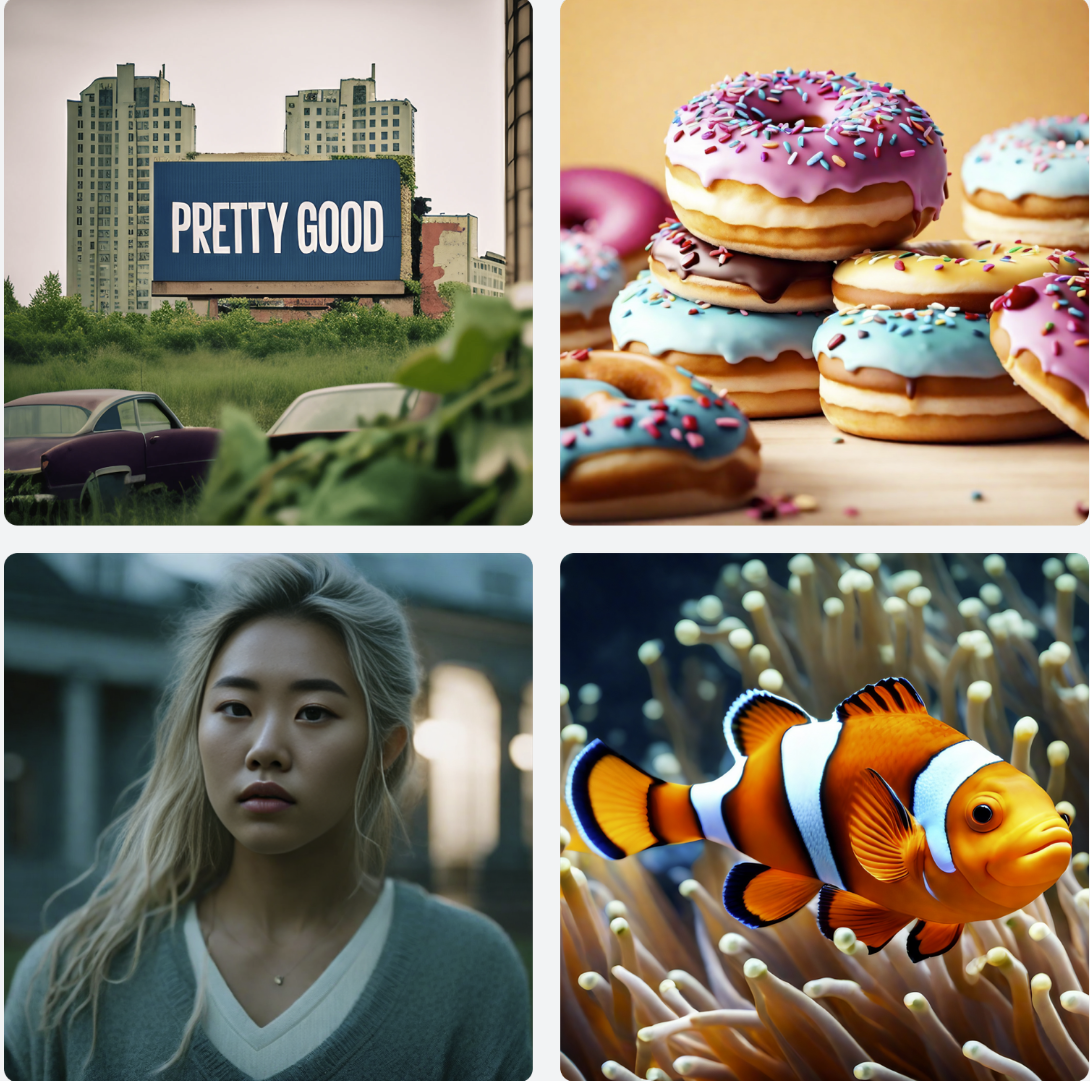
\includegraphics[width=0.95\textwidth]
			{assets/stable}
		\end{figure}
	\end{columns}
\end{frame}

\begin{frame}{Introduction}
\framesubtitle{The promising future of foundation model}
	\begin{figure}
		\centering
		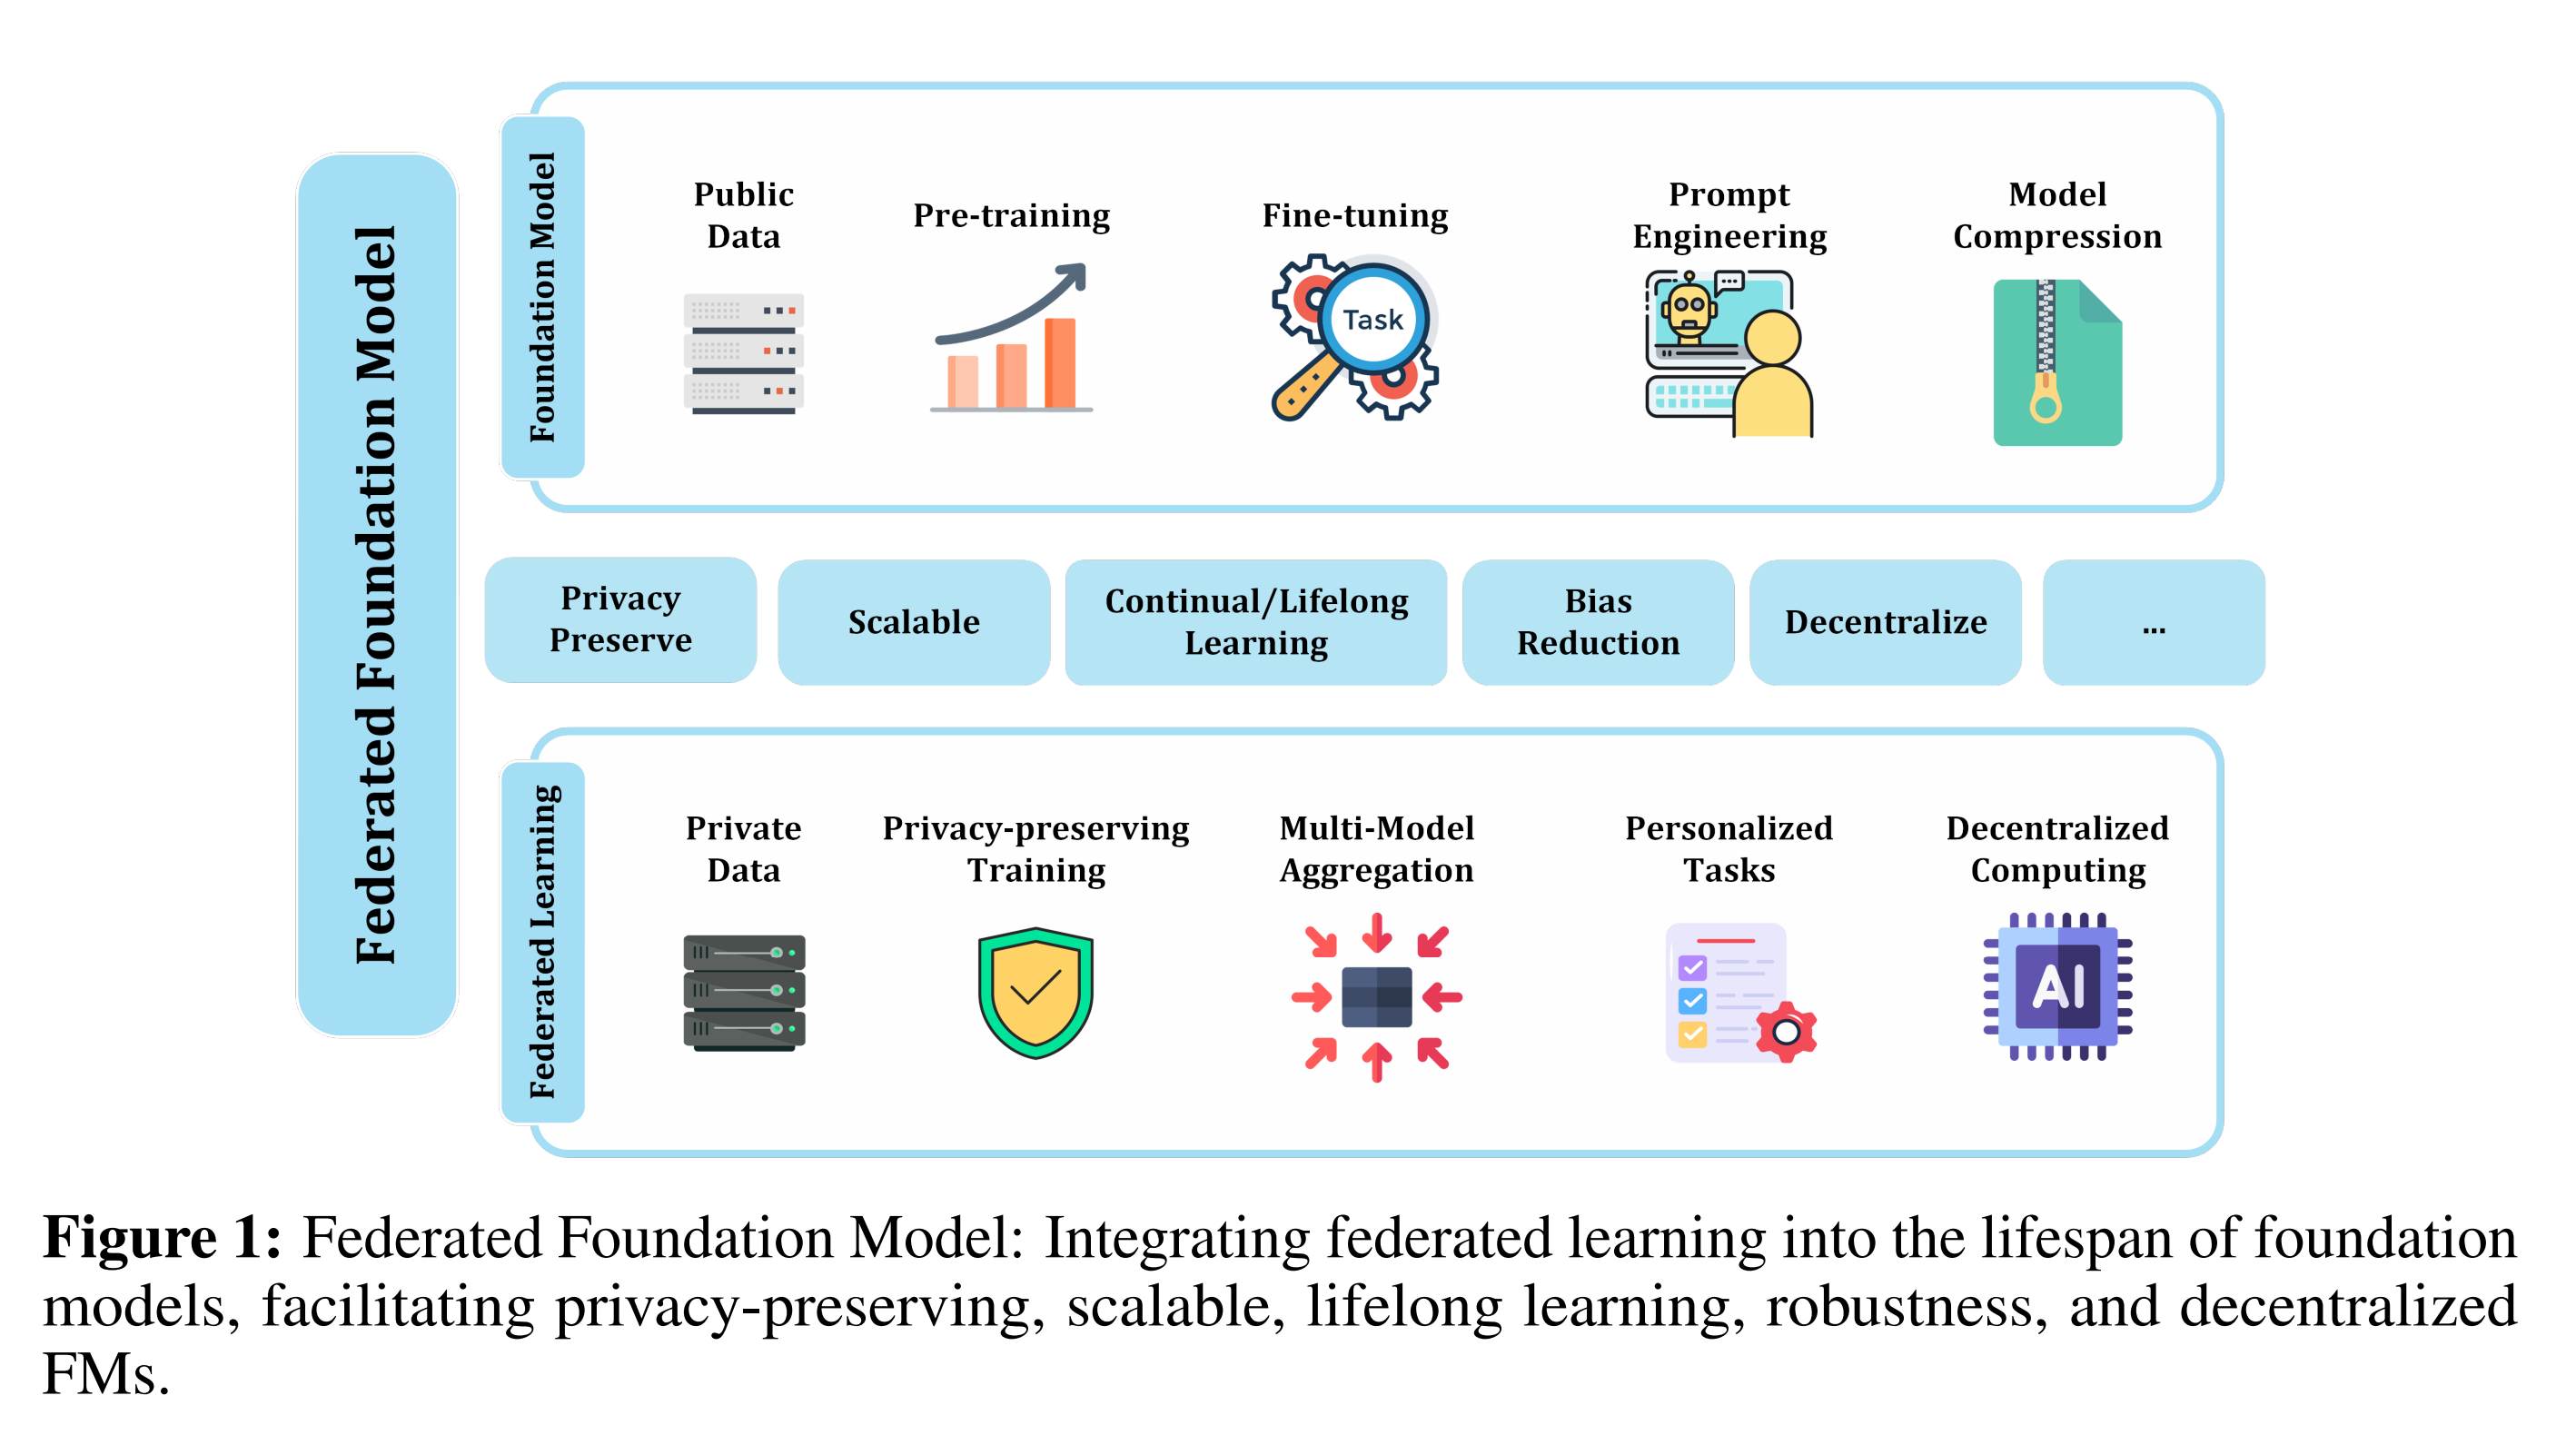
\includegraphics[width=0.8\textwidth]
		{assets/FM}
	\end{figure}
	
\end{frame}

\section{Method}

\begin{frame}{Method}
\framesubtitle{The previous way of using foundation models}
\begin{figure}
			\centering
			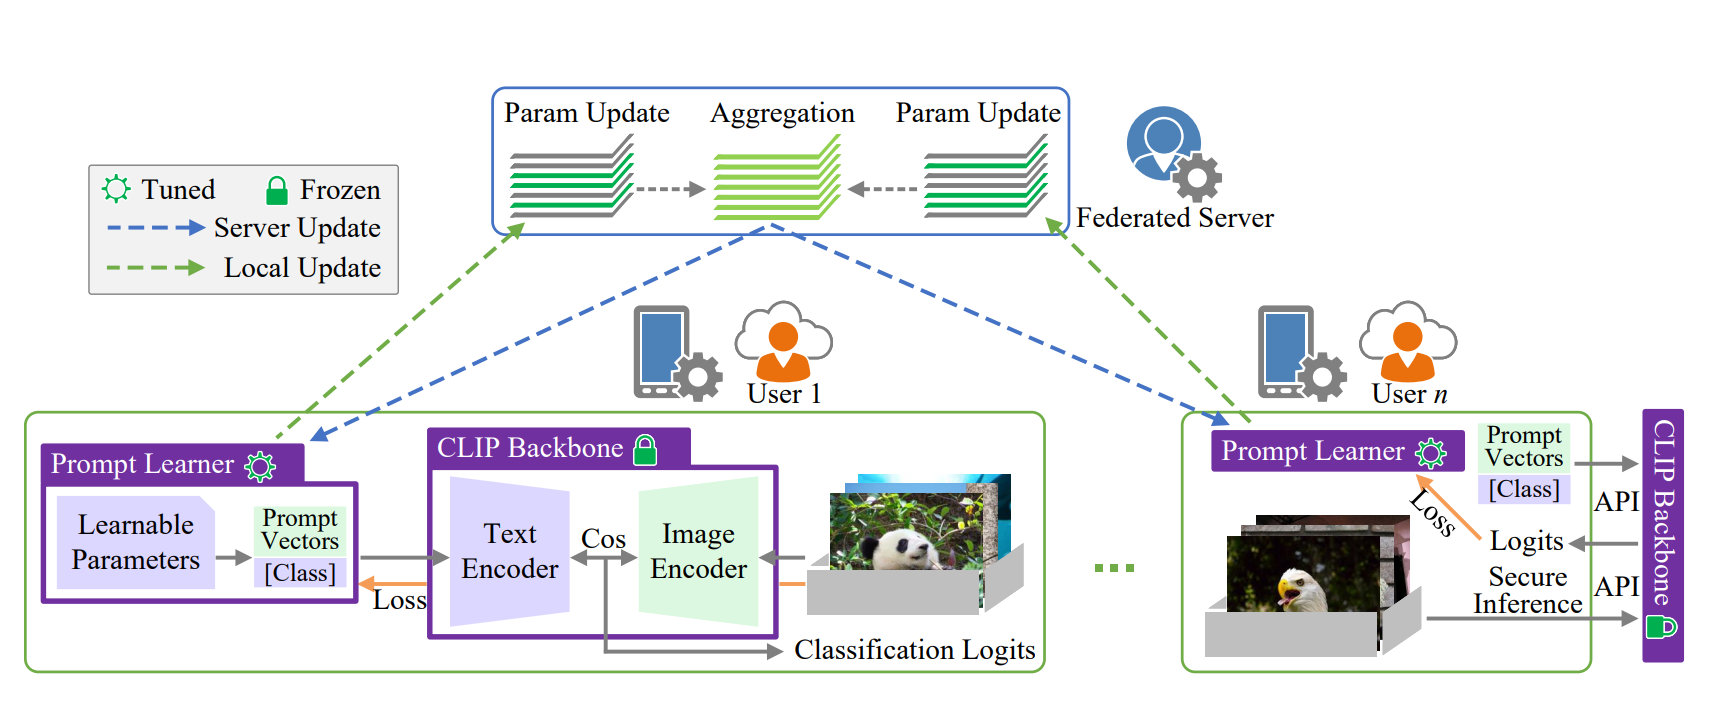
\includegraphics[width=0.95\textwidth]
			{assets/promptfl}
	\end{figure}
	PROMPTFL: Let Federated Participants Cooperatively Learn Prompts Instead of Models
\end{frame}

\begin{frame}{Method}
\framesubtitle{Main difference}
	\begin{itemize}
		\item Their methods transmit features or parameters, while our federated generative learning framework \textbf{transmits prompts which require less communication while are better at privacy-preserving}.
		\item Our framework is based on\textbf{ shared foundation generative models}, while theirs are based on the shared foundation classification models.
	\end{itemize}
\end{frame}

\begin{frame}{Method}
\framesubtitle{Federated Generative Learning Diagram}
\begin{figure}
			\centering
			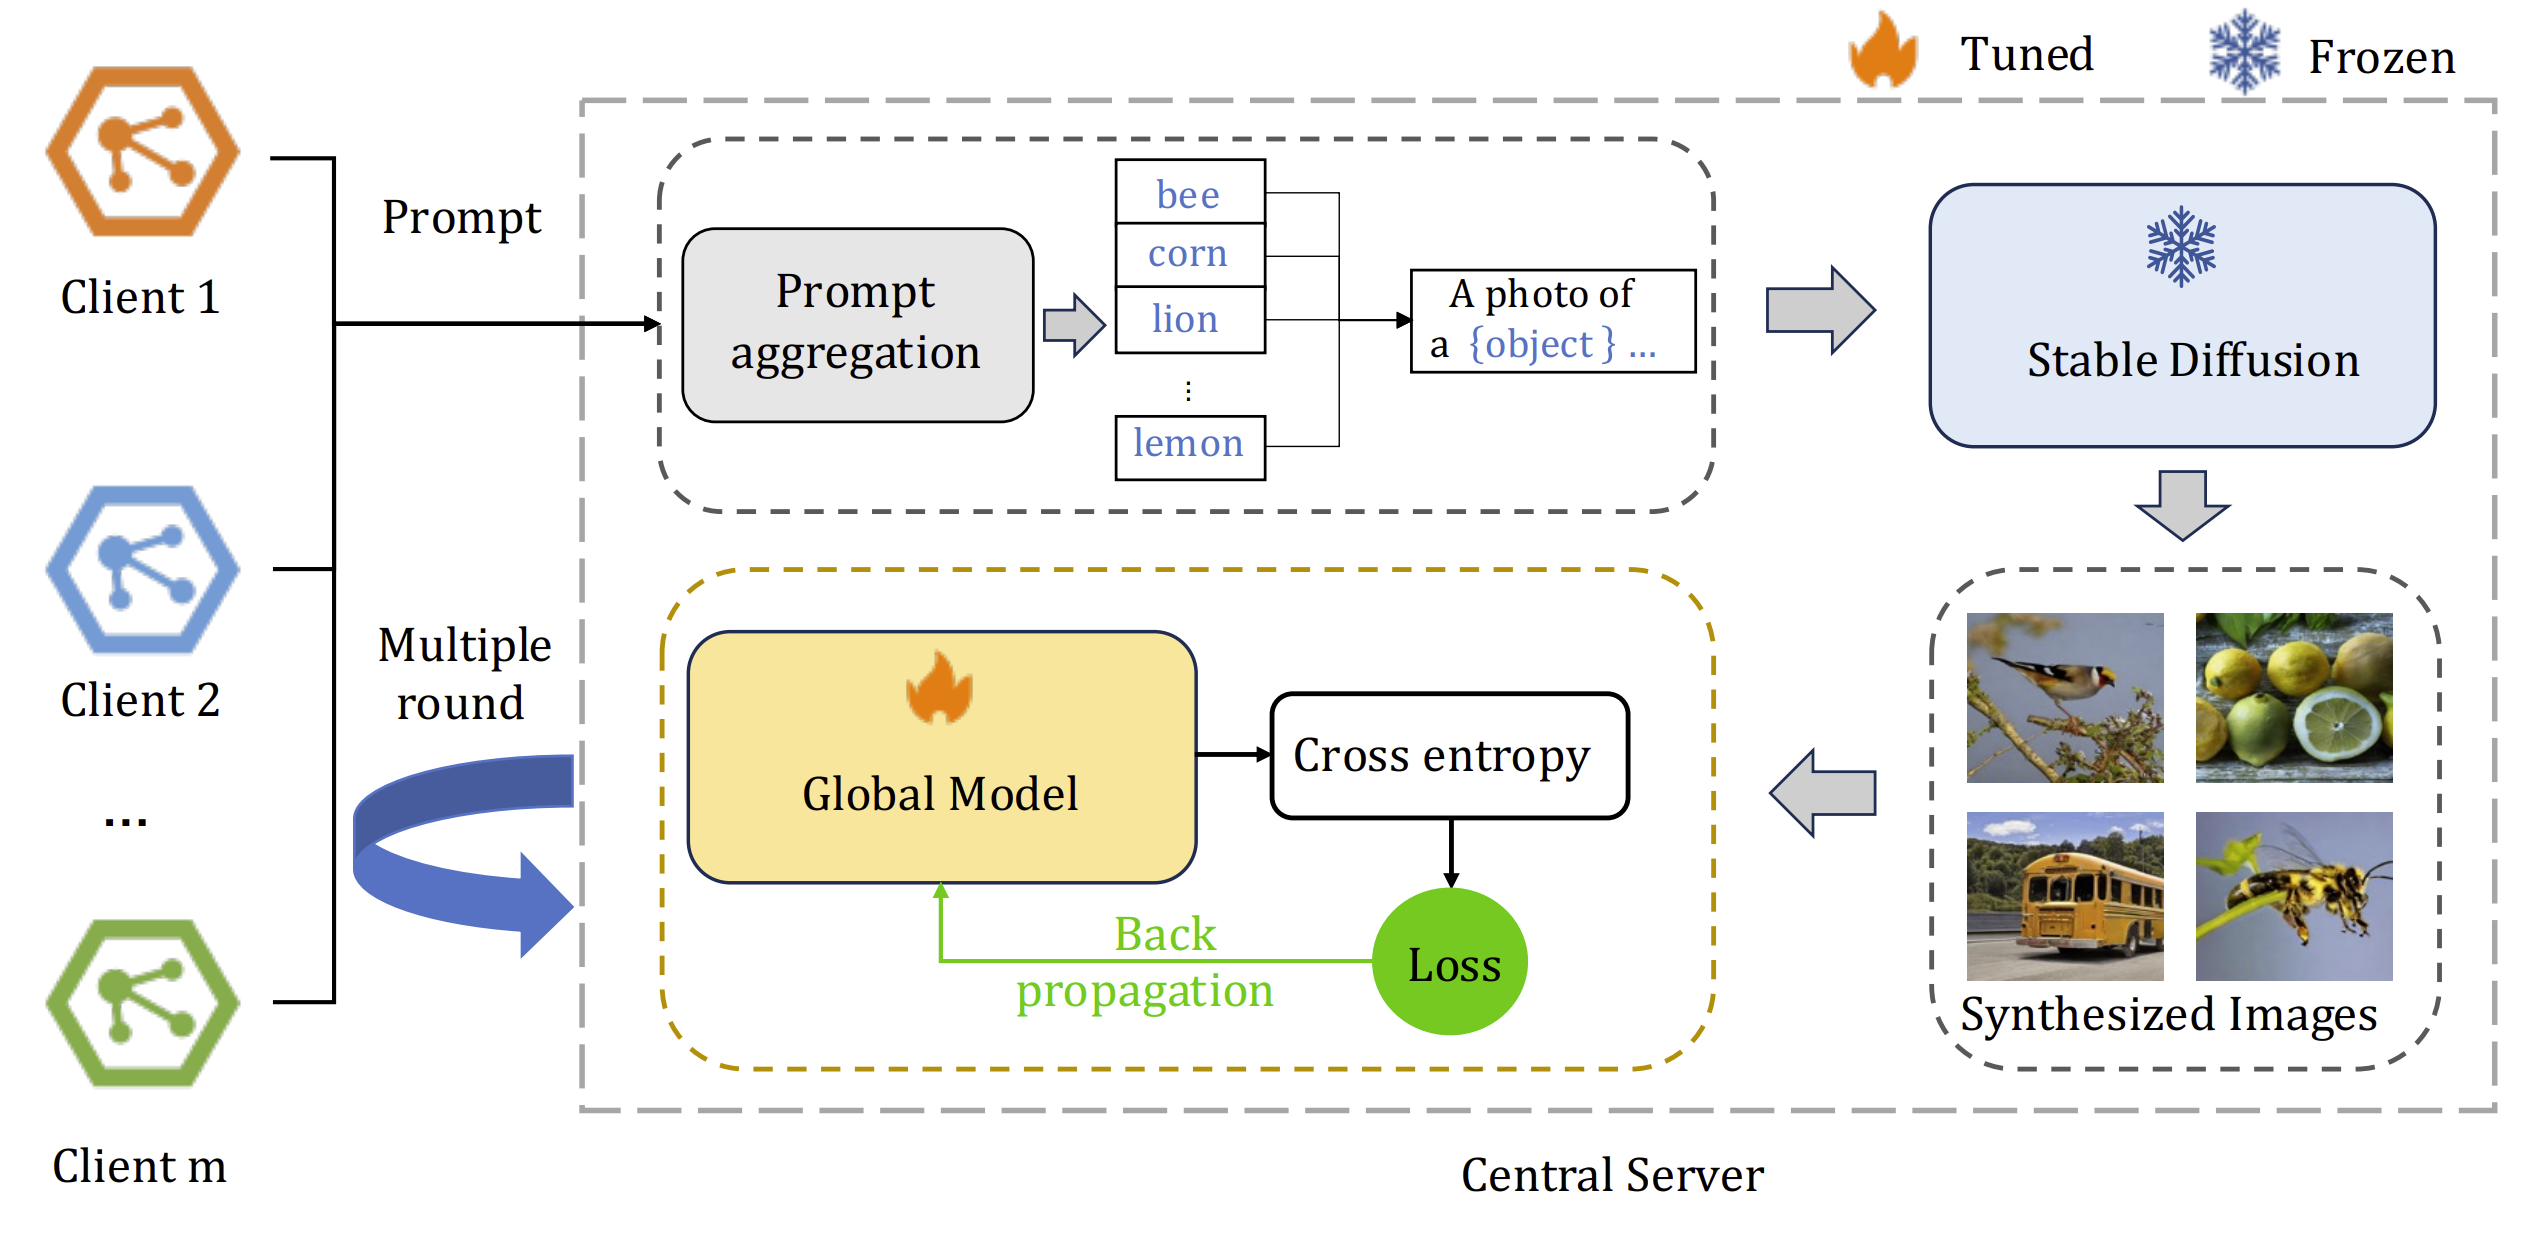
\includegraphics[width=0.9\textwidth]
			{assets/diagram}
		\end{figure}
\end{frame}


\begin{frame}{Method}
\framesubtitle{Prompt generation in clients}
This framework can implement one-shot FL, and the clients do not need to train models locally
\begin{figure}
			\centering
			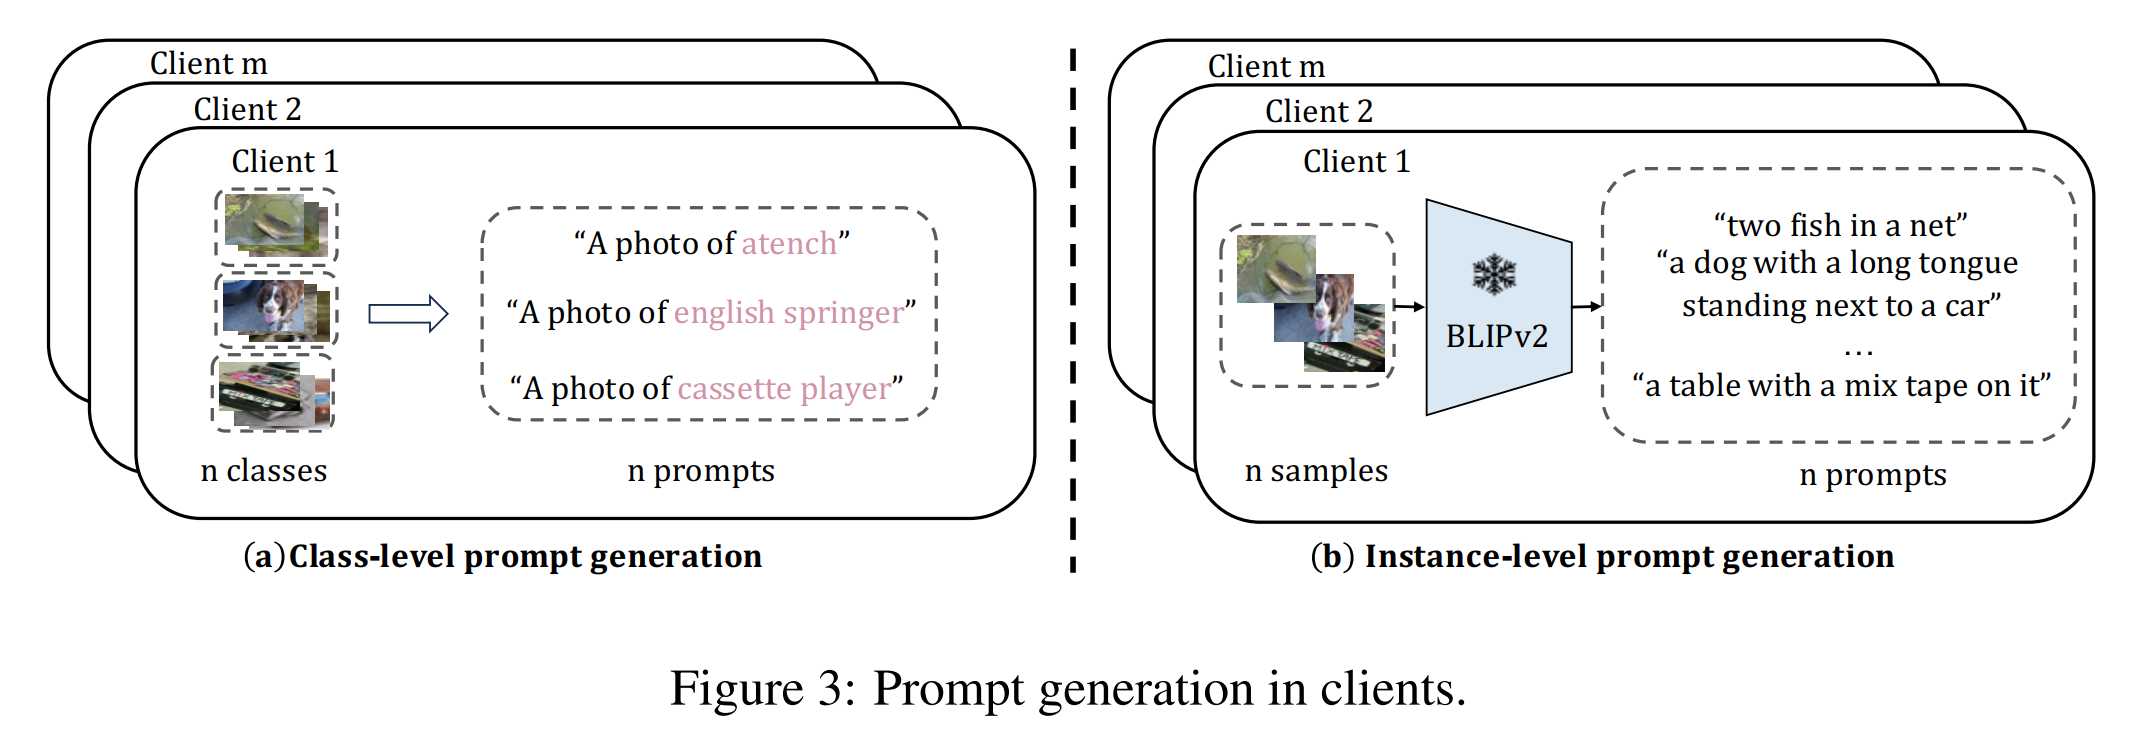
\includegraphics[width=1.0\textwidth]
			{assets/prompt}
		\end{figure}
\end{frame}

\begin{frame}{Method}
\framesubtitle{Training set synthesis}
After receiving all prompts, the server synthesizes every training sample $s_i$ by prompting the pretrained Stable Diffusion with each $p_i$ as follows:
$$
\boldsymbol{s}_i=G\left(\boldsymbol{z}_i, \boldsymbol{p}_i\right)=\sqrt{\beta} \sum_{t=1}^T \sqrt{1-\beta^t} \cdot \frac{1}{\sqrt{T}} \cdot G_{\boldsymbol{\vartheta}_t}\left(\boldsymbol{z}_i, \boldsymbol{p}_i\right)
$$
\begin{itemize}
		\item $z_i$ is a random noise vector
		\item $p_i$ is the prompt
		\item $G_{\theta_t}$ is the denoising network parameterized with $\theta_t$ at time step $t$
		\item $\beta$ controls the trade-off between image quality and diversity
		\item $T$ is the number of diffusion steps
\end{itemize}
\end{frame}

\section{Experiment}

\begin{frame}{Experiment}
\framesubtitle{Model updating}
	\begin{itemize}
	\item ONE-SHOT UPDATING: \\
	After obtaining the synthetic training set, jointly train the model in the server.
	\item MULTI-ROUND UPDATING: \\
	Implement multi-round communication like traditional FL methods, which can
	bring further performance improvement
		\begin{itemize}
		\item Without Synthetic Data: \\
		After
		locally fine-tuning, the server collect updated models from all clients for model aggregation
		\item With Synthetic Data: \\
		Fine-tuning the
		aggregated model on synthetic training set in every-round communication can \textbf{remarkablely improve
		the performance when the data distribution is extremely imbalanced} in clients
		\end{itemize}
	\end{itemize}
\end{frame}

\begin{frame}{Experiment}
\framesubtitle{Experiment Result}
	\begin{figure}
	\centering
	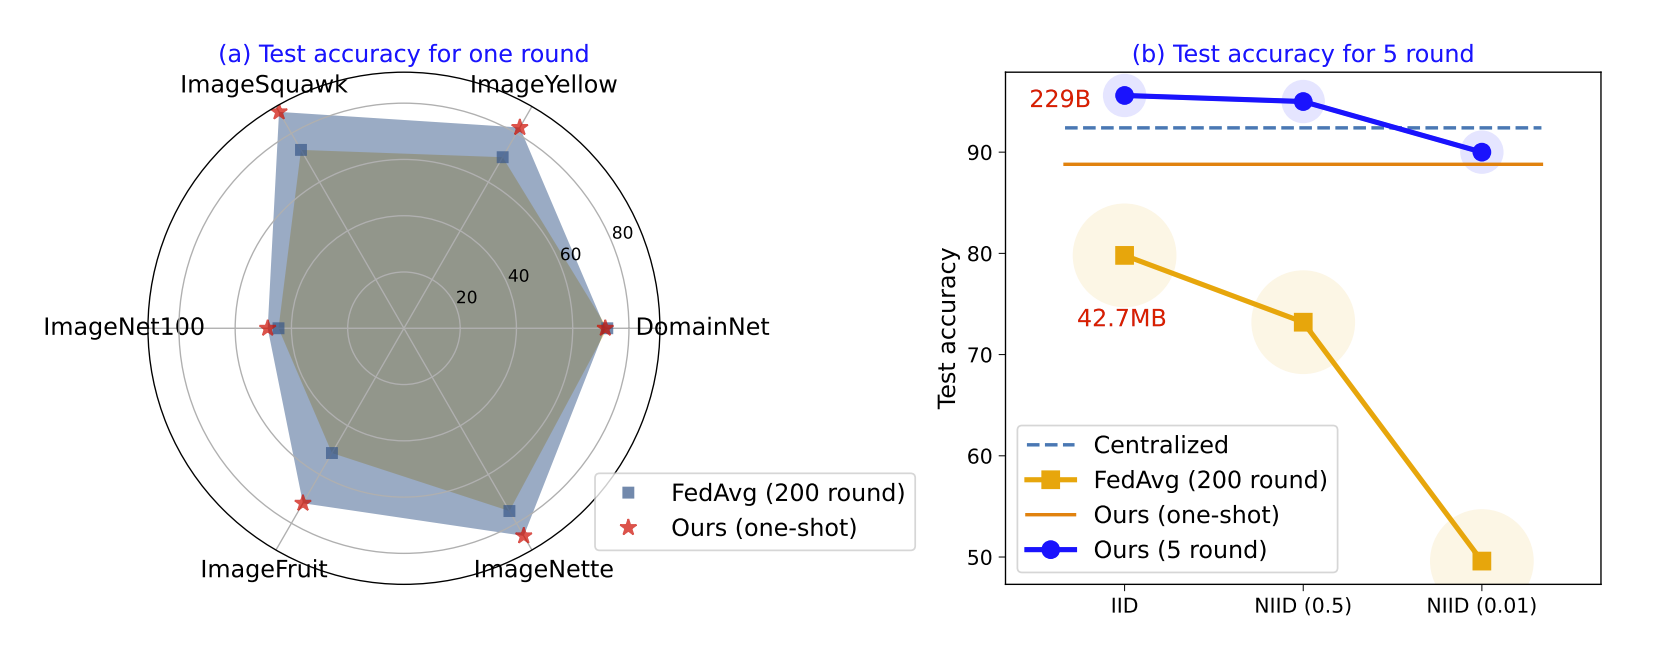
\includegraphics[width=1.0\textwidth]
	{assets/performance}
	\end{figure}
\end{frame}

\begin{frame}{Experiment}
\framesubtitle{Experiment Result}
	\begin{figure}
	\centering
	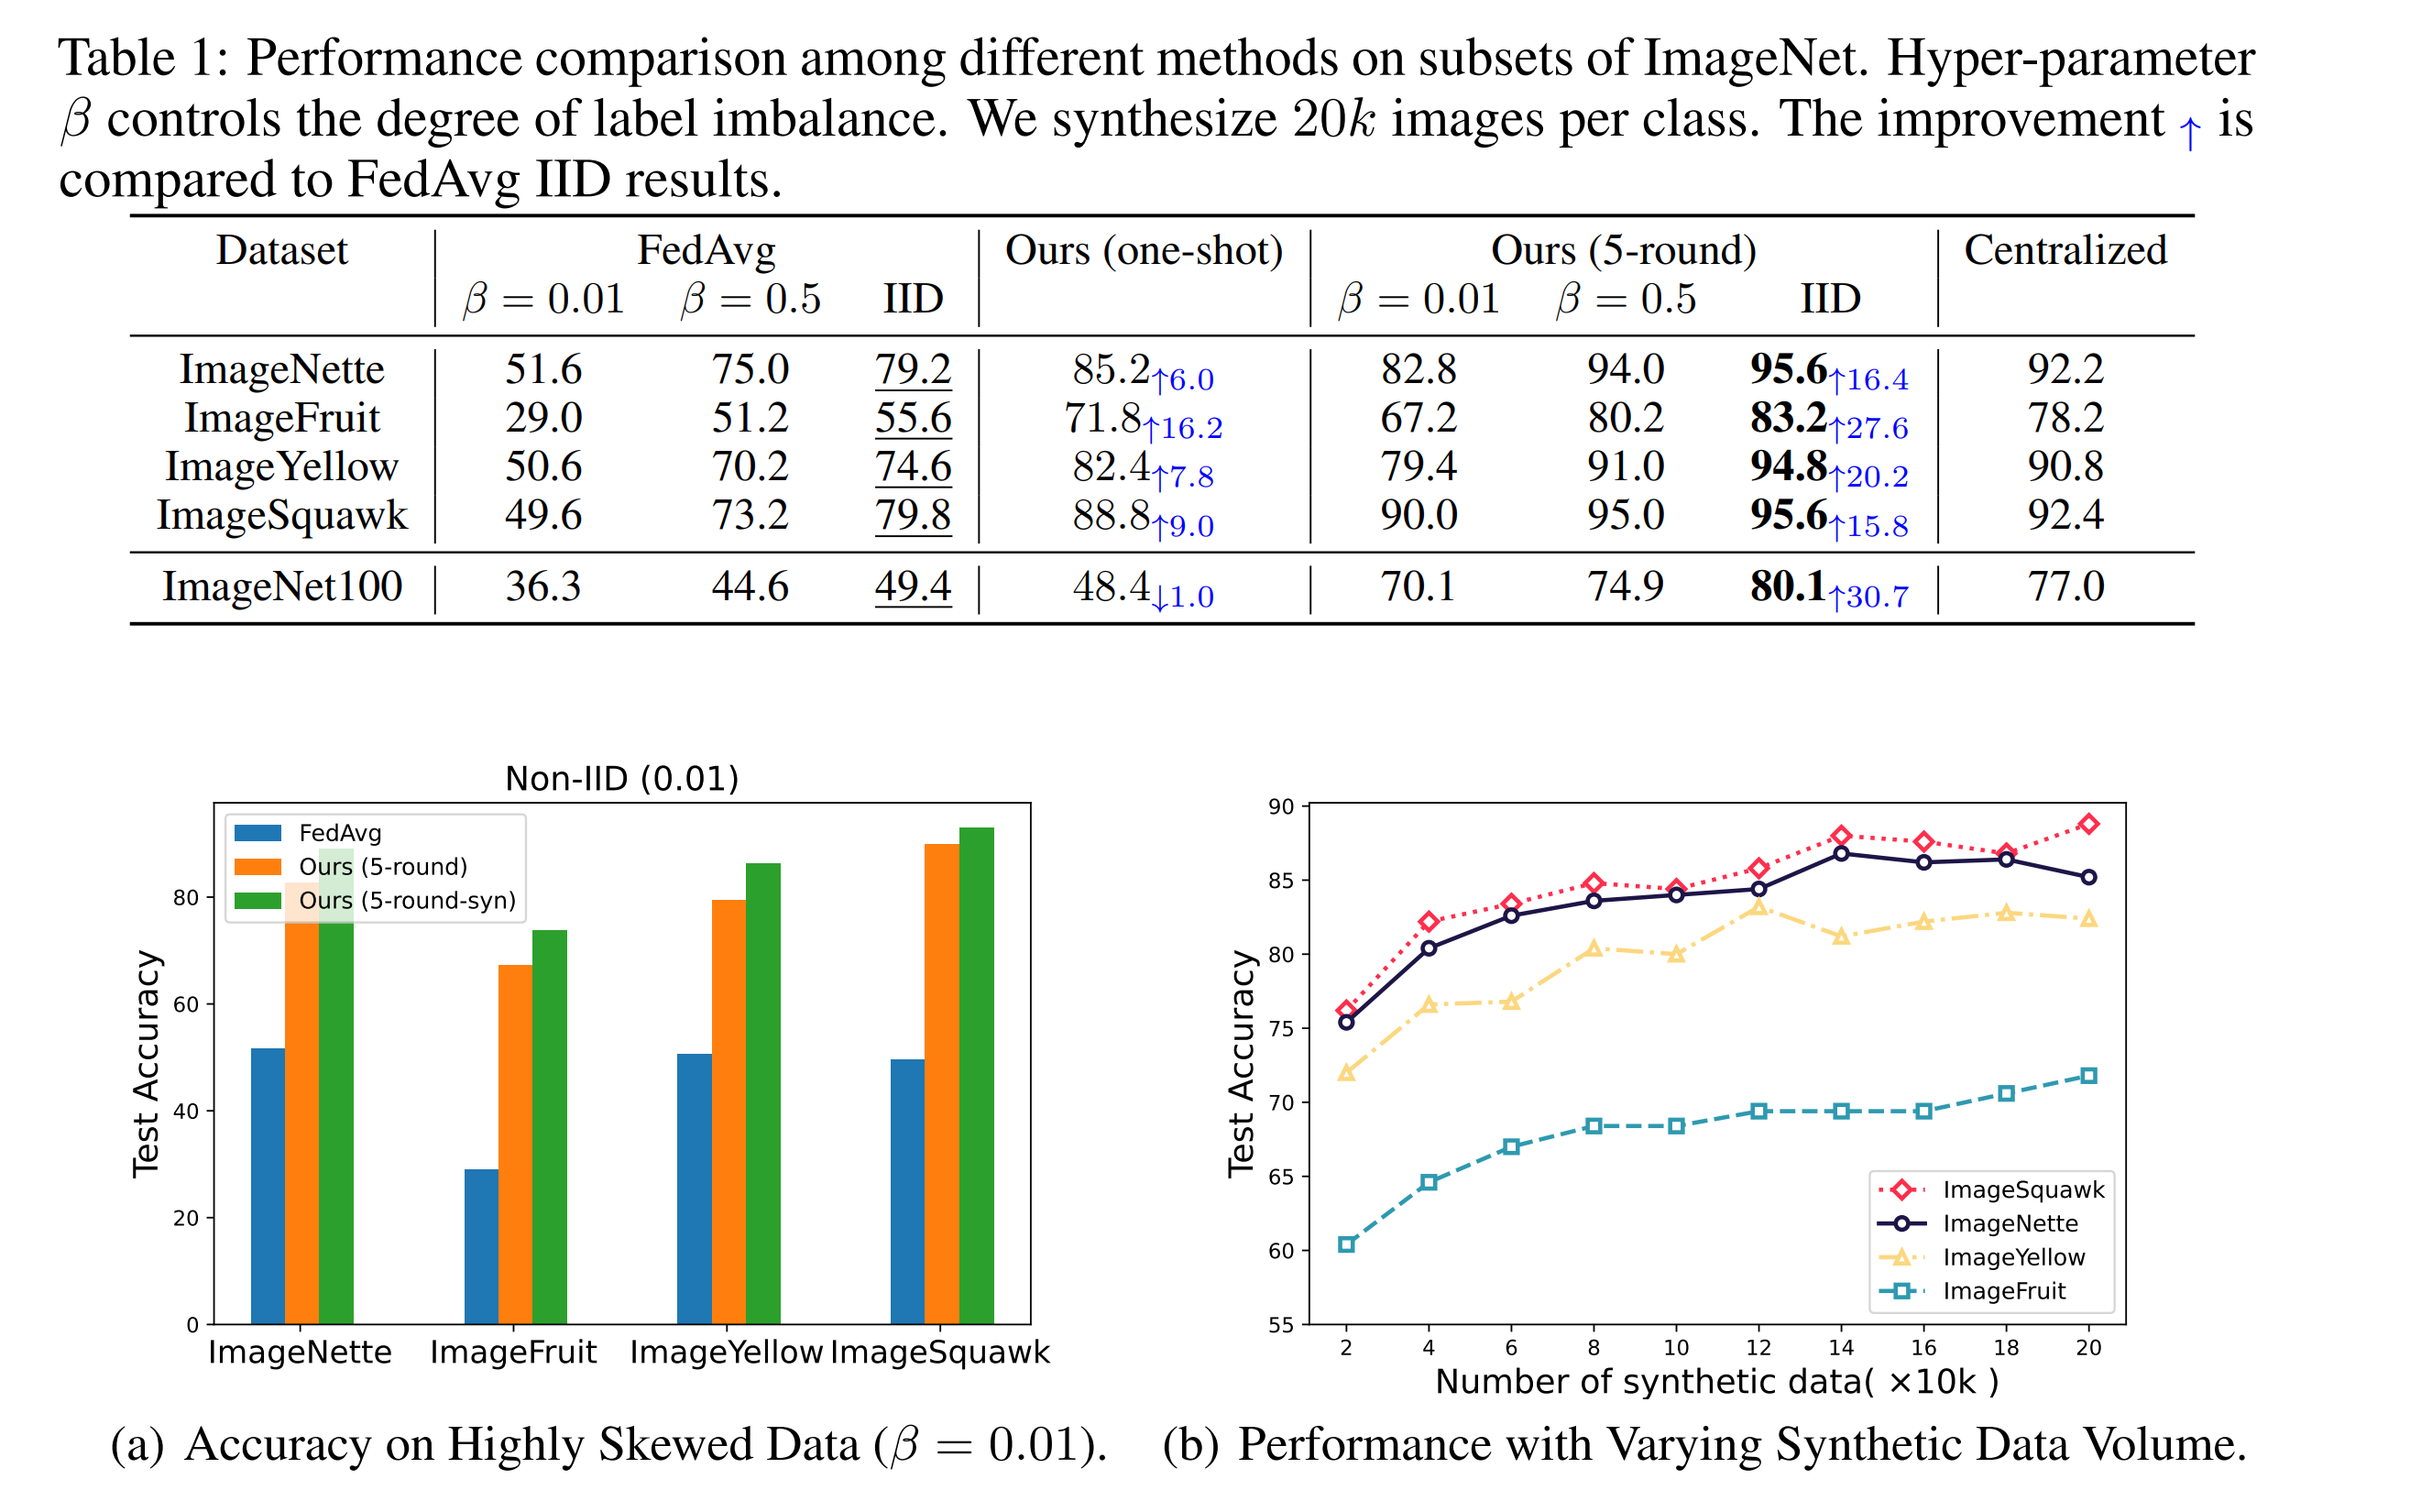
\includegraphics[width=0.7\textwidth]
	{assets/result}
	\end{figure}
\end{frame}

\begin{frame}{Ablation Study}
\framesubtitle{Class-level Prompts versus Instance-level Prompts}
	\begin{figure}
	\centering
	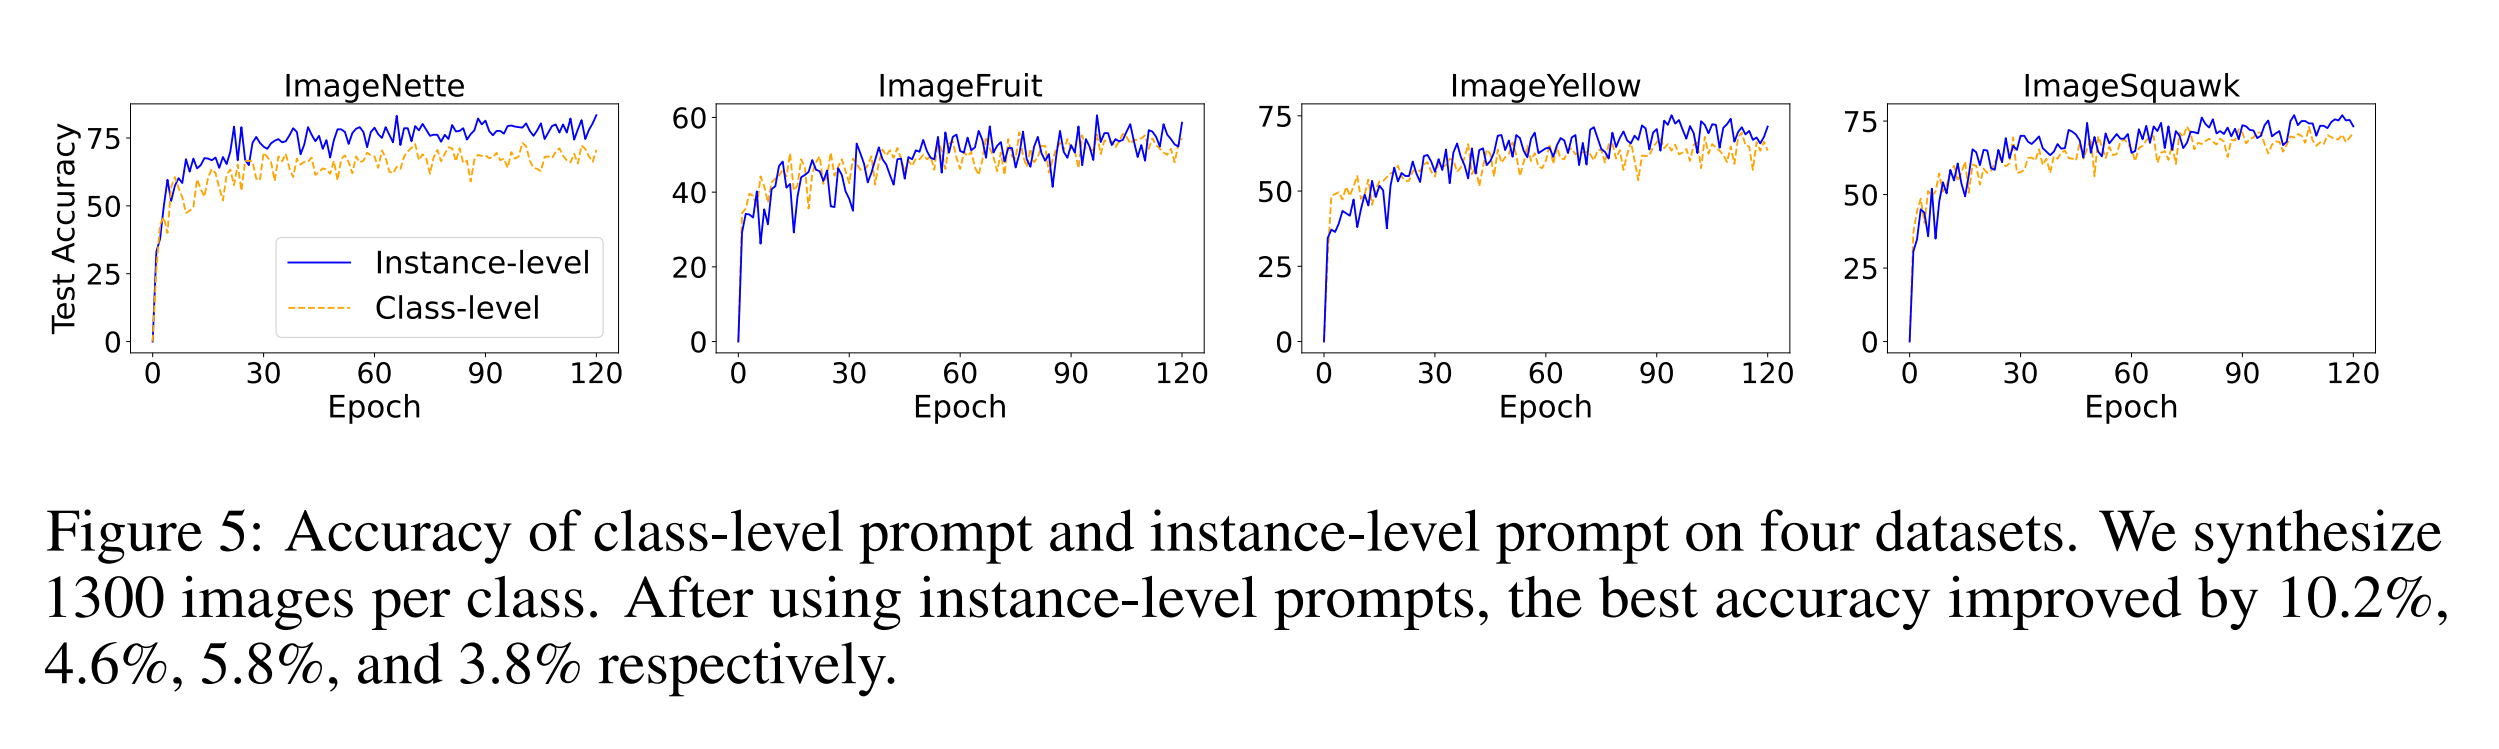
\includegraphics[width=0.95\textwidth]
	{assets/ablation}
	\end{figure}
\end{frame}



\begin{frame}{Ablation Study}
\framesubtitle{Limitation on Domainnet}
	\begin{figure}
	\centering
	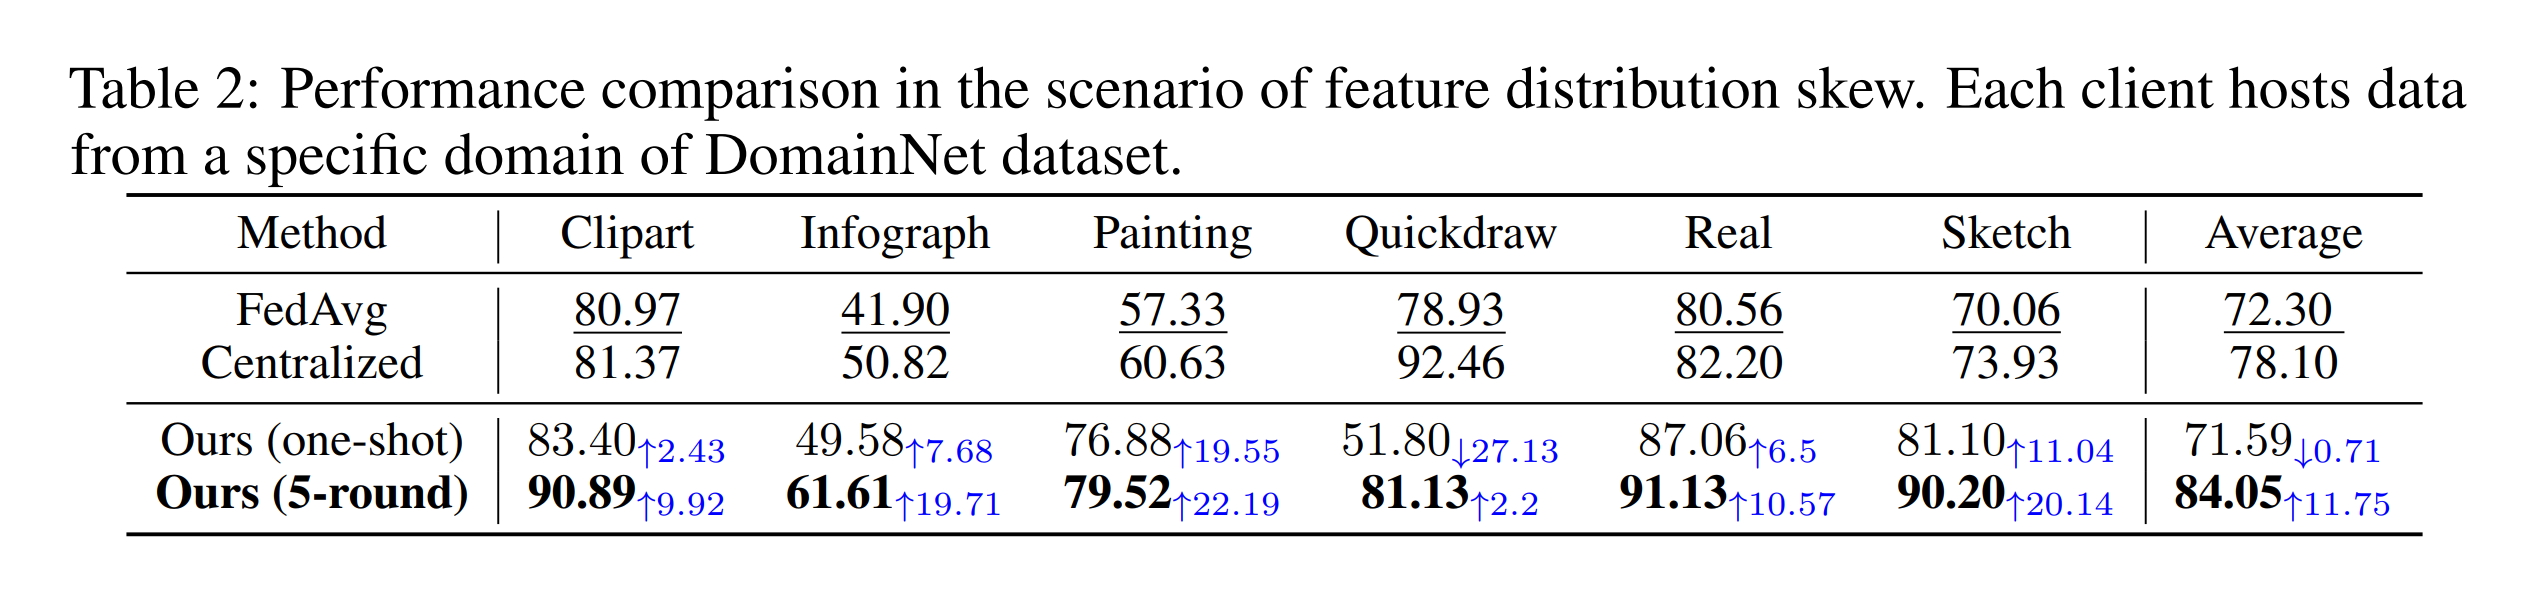
\includegraphics[width=0.9\textwidth]
	{assets/domainnet}
	\end{figure}
\end{frame}

\begin{frame}{Ablation Study}
\framesubtitle{Ablation Study}
	\begin{figure}
	\centering
	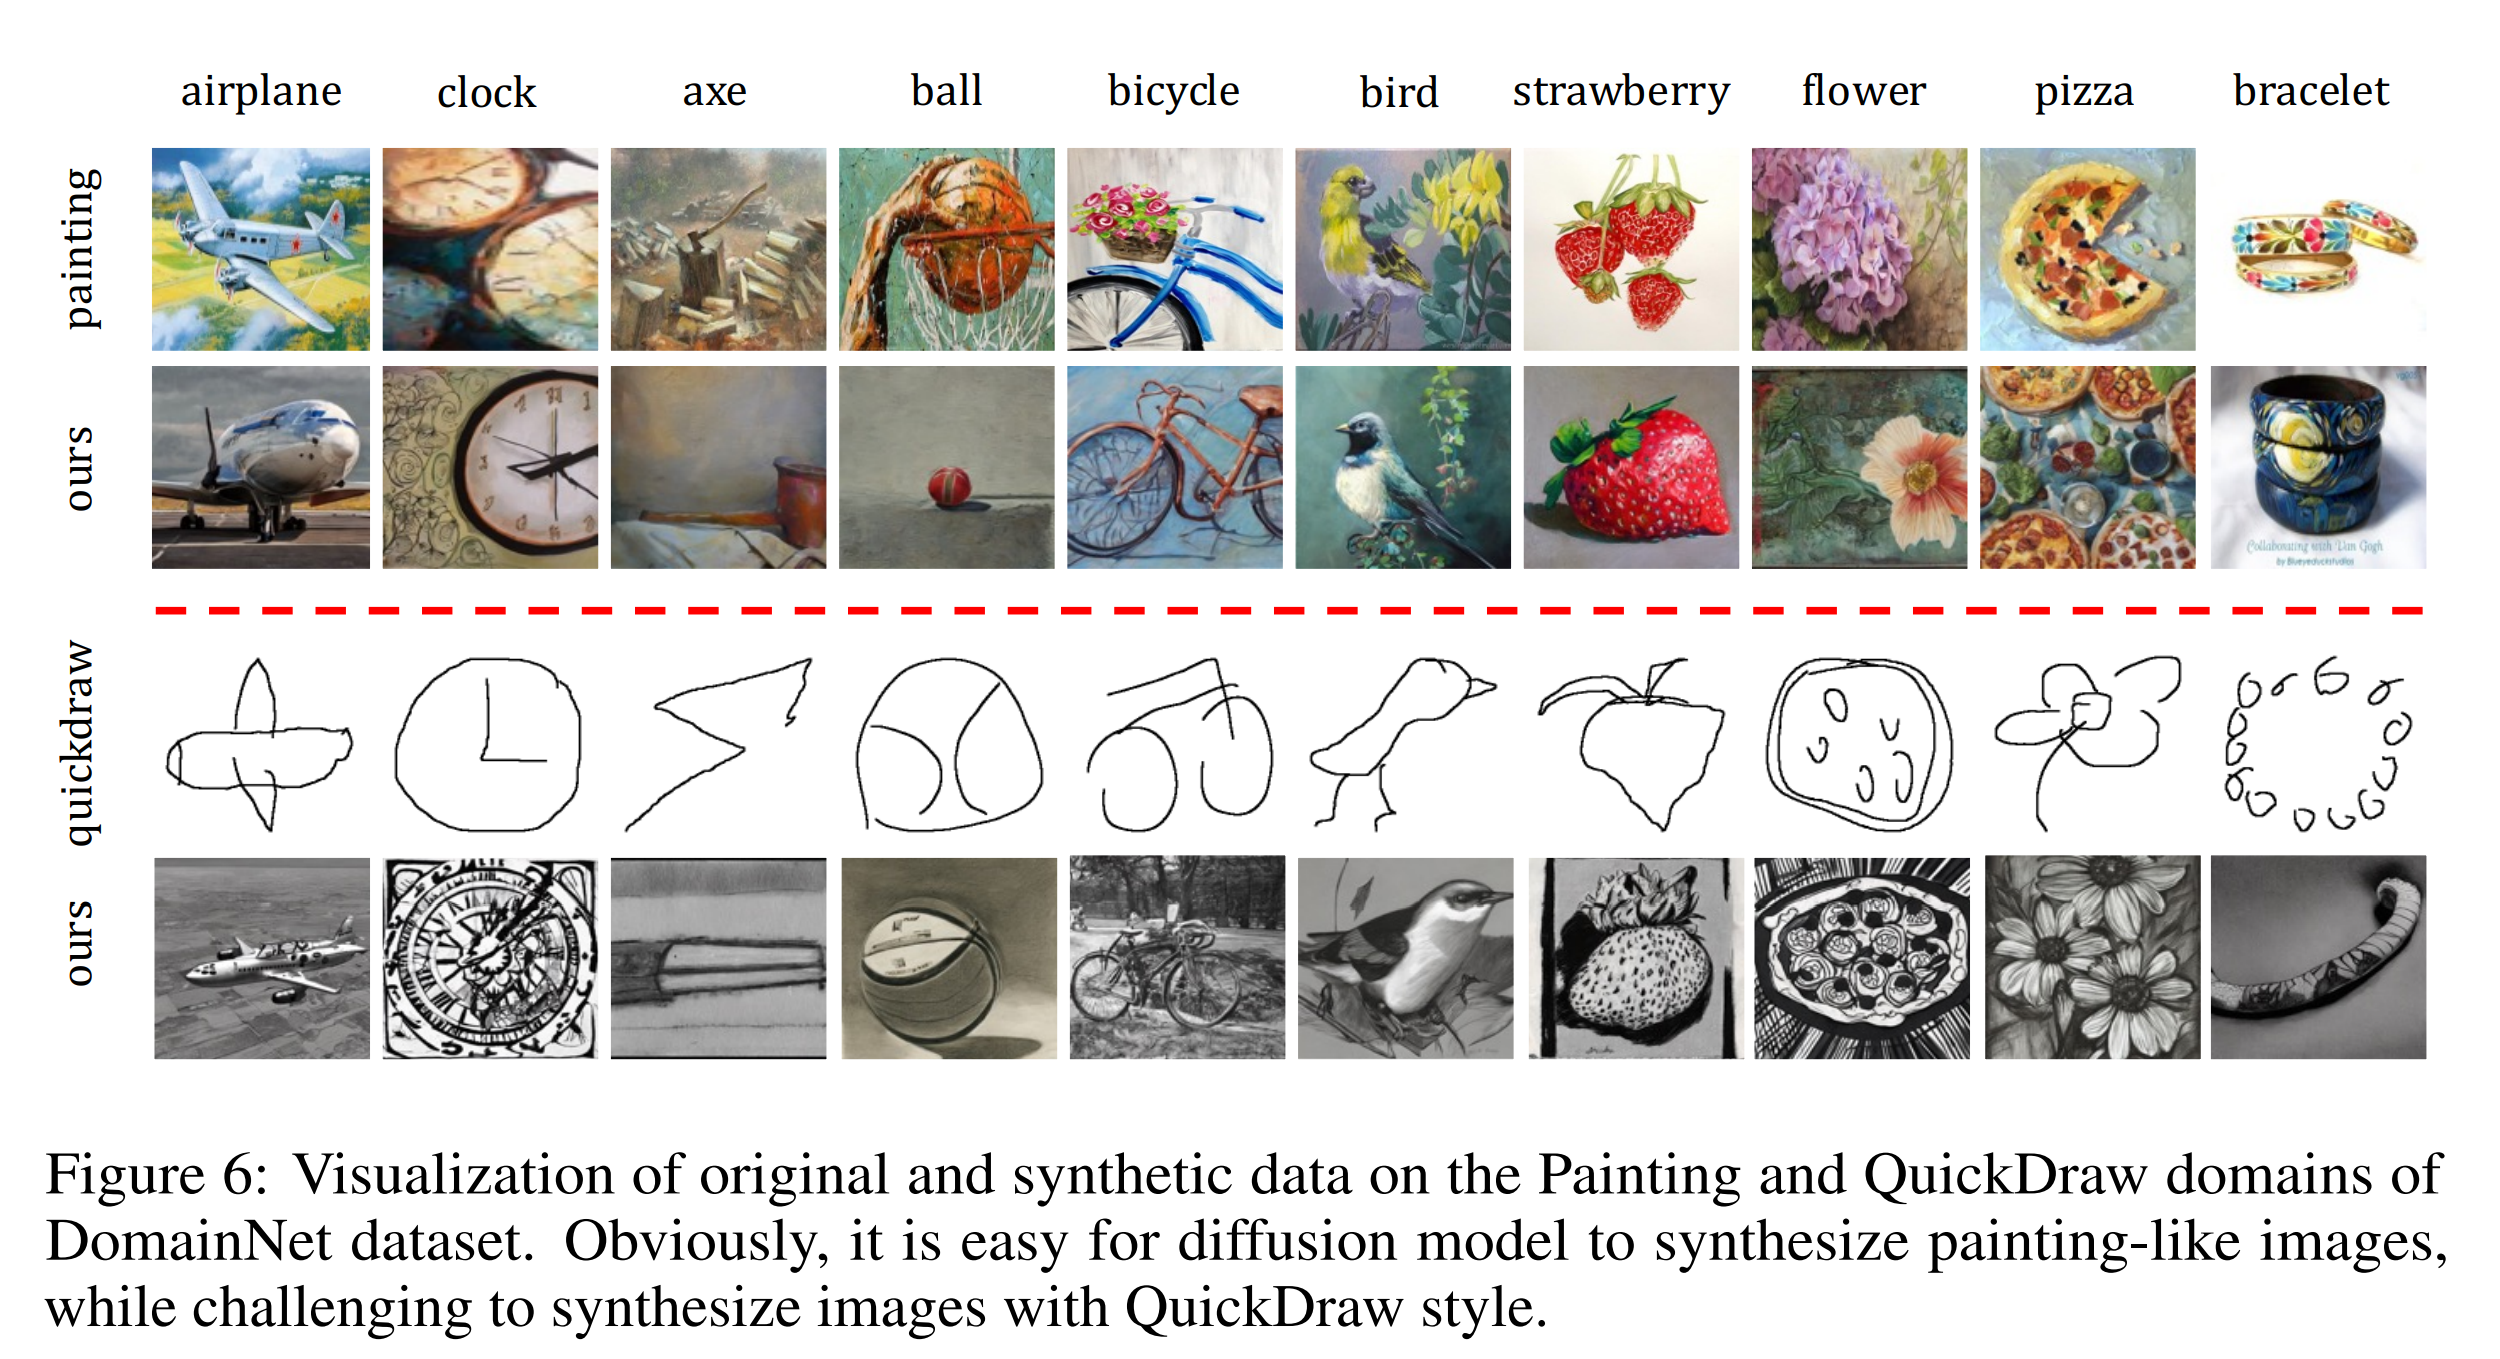
\includegraphics[width=0.85\textwidth]
	{assets/quickdraw}
	\end{figure}
\end{frame}

\section{Discussion}

\begin{frame}
\frametitle{Discussion}
\framesubtitle{Detecting Content Replication and Memorization}
	\begin{figure}
	\centering
	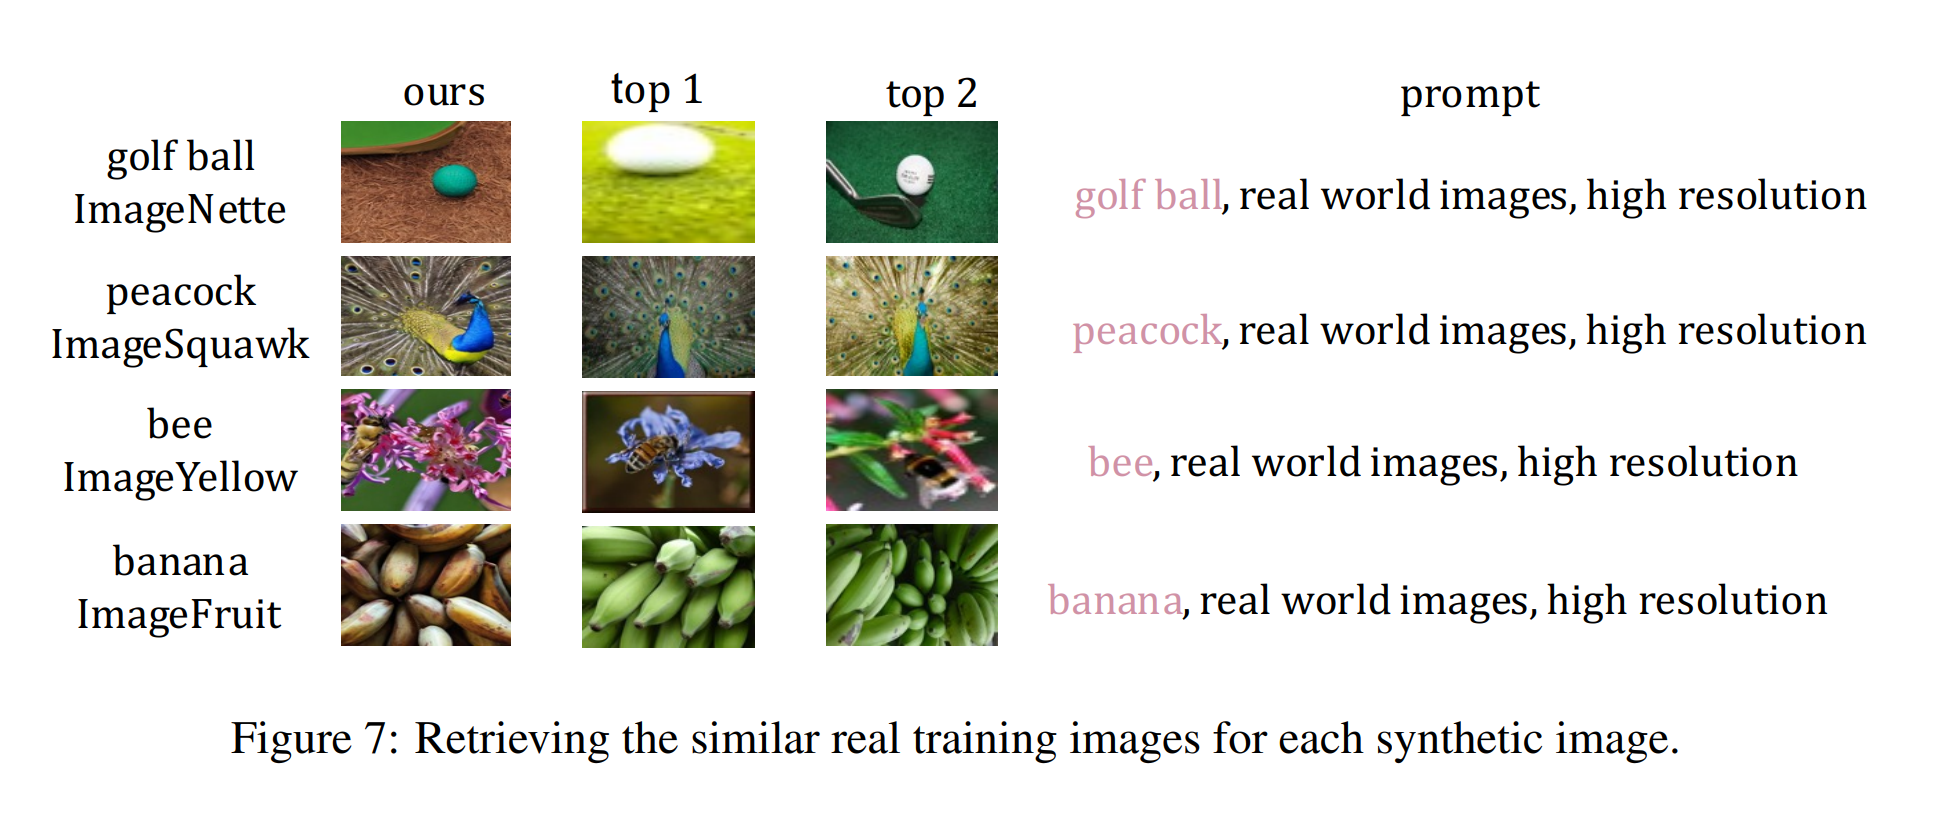
\includegraphics[width=0.7\textwidth]
	{assets/replication}
	\end{figure}
	It is obvious that these images exhibit no noteworthy similarities in terms of both background and
	foreground. This observation verifies that our method \textbf{does not compromise the privacy of the client's
	private data.}
\end{frame}

\begin{frame}
\frametitle{Discussion}
\framesubtitle{Membership Inference Attack}
	\begin{figure}
	\centering
	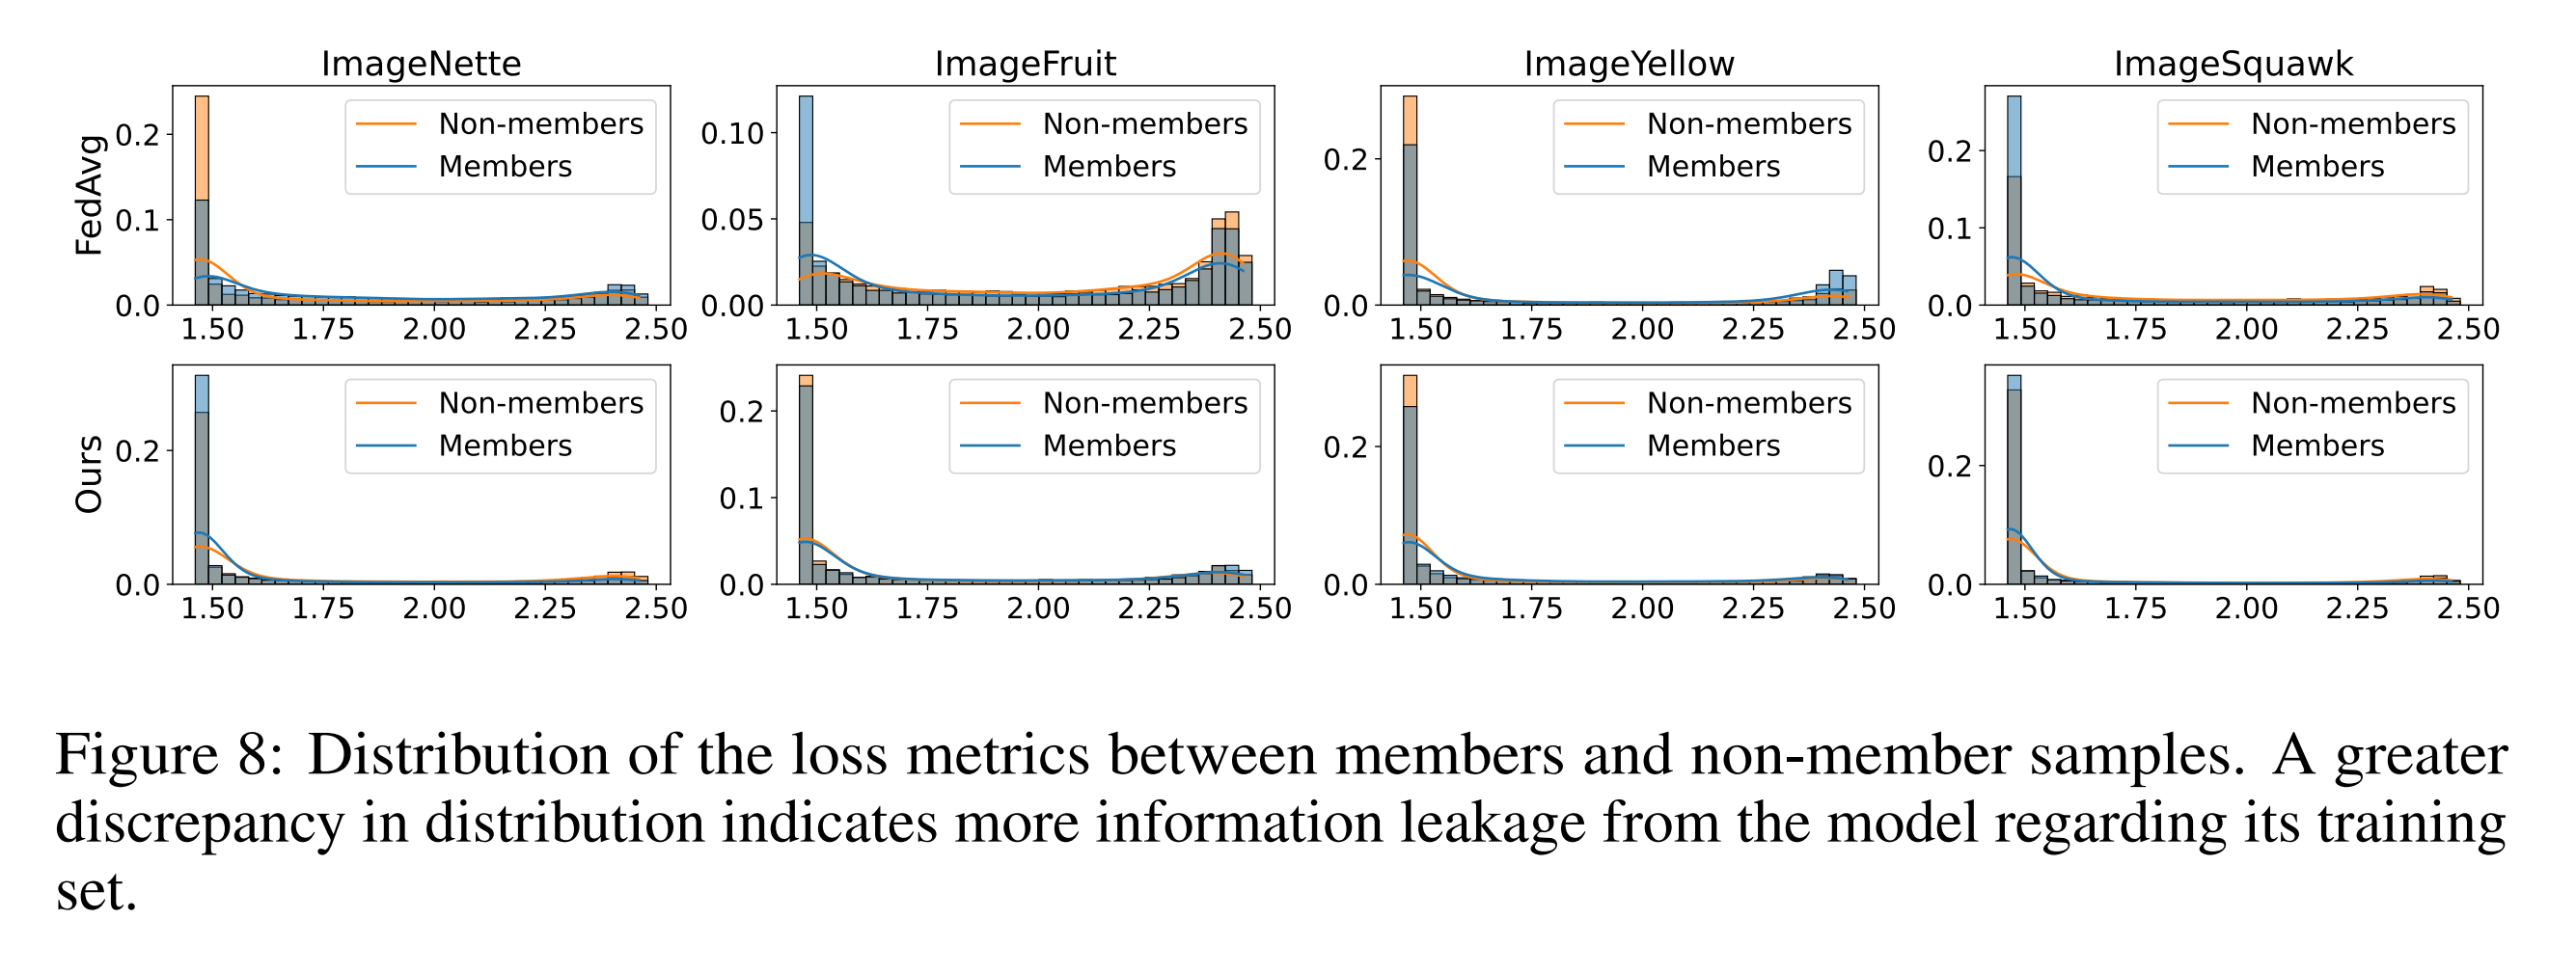
\includegraphics[width=0.85\textwidth]
	{assets/MIA}
	\end{figure}
	Membership Inference Attack is a type of attack that aims to determine whether a sample belongs to the training dataset of a machine learning model or not.
\end{frame}



\begin{frame}
\frametitle{Discussion}
\framesubtitle{Summary}
A pioneering framework for Federated Learning, which transmits prompts associated with distributed training data between clients and
the server.
\begin{itemize}
\item The usage of prompts and foundation model.
\item Interesting experiment design.
\item The discussion of privacy protection.
\end{itemize}
\end{frame}

\section{Take Home Message}
\begin{frame}
\frametitle{Ray Tune}
\framesubtitle{Fast and easy distributed hyperparameter tuning}

\begin{columns}
	\column{0.7\textwidth}
		\begin{figure}
			\centering
			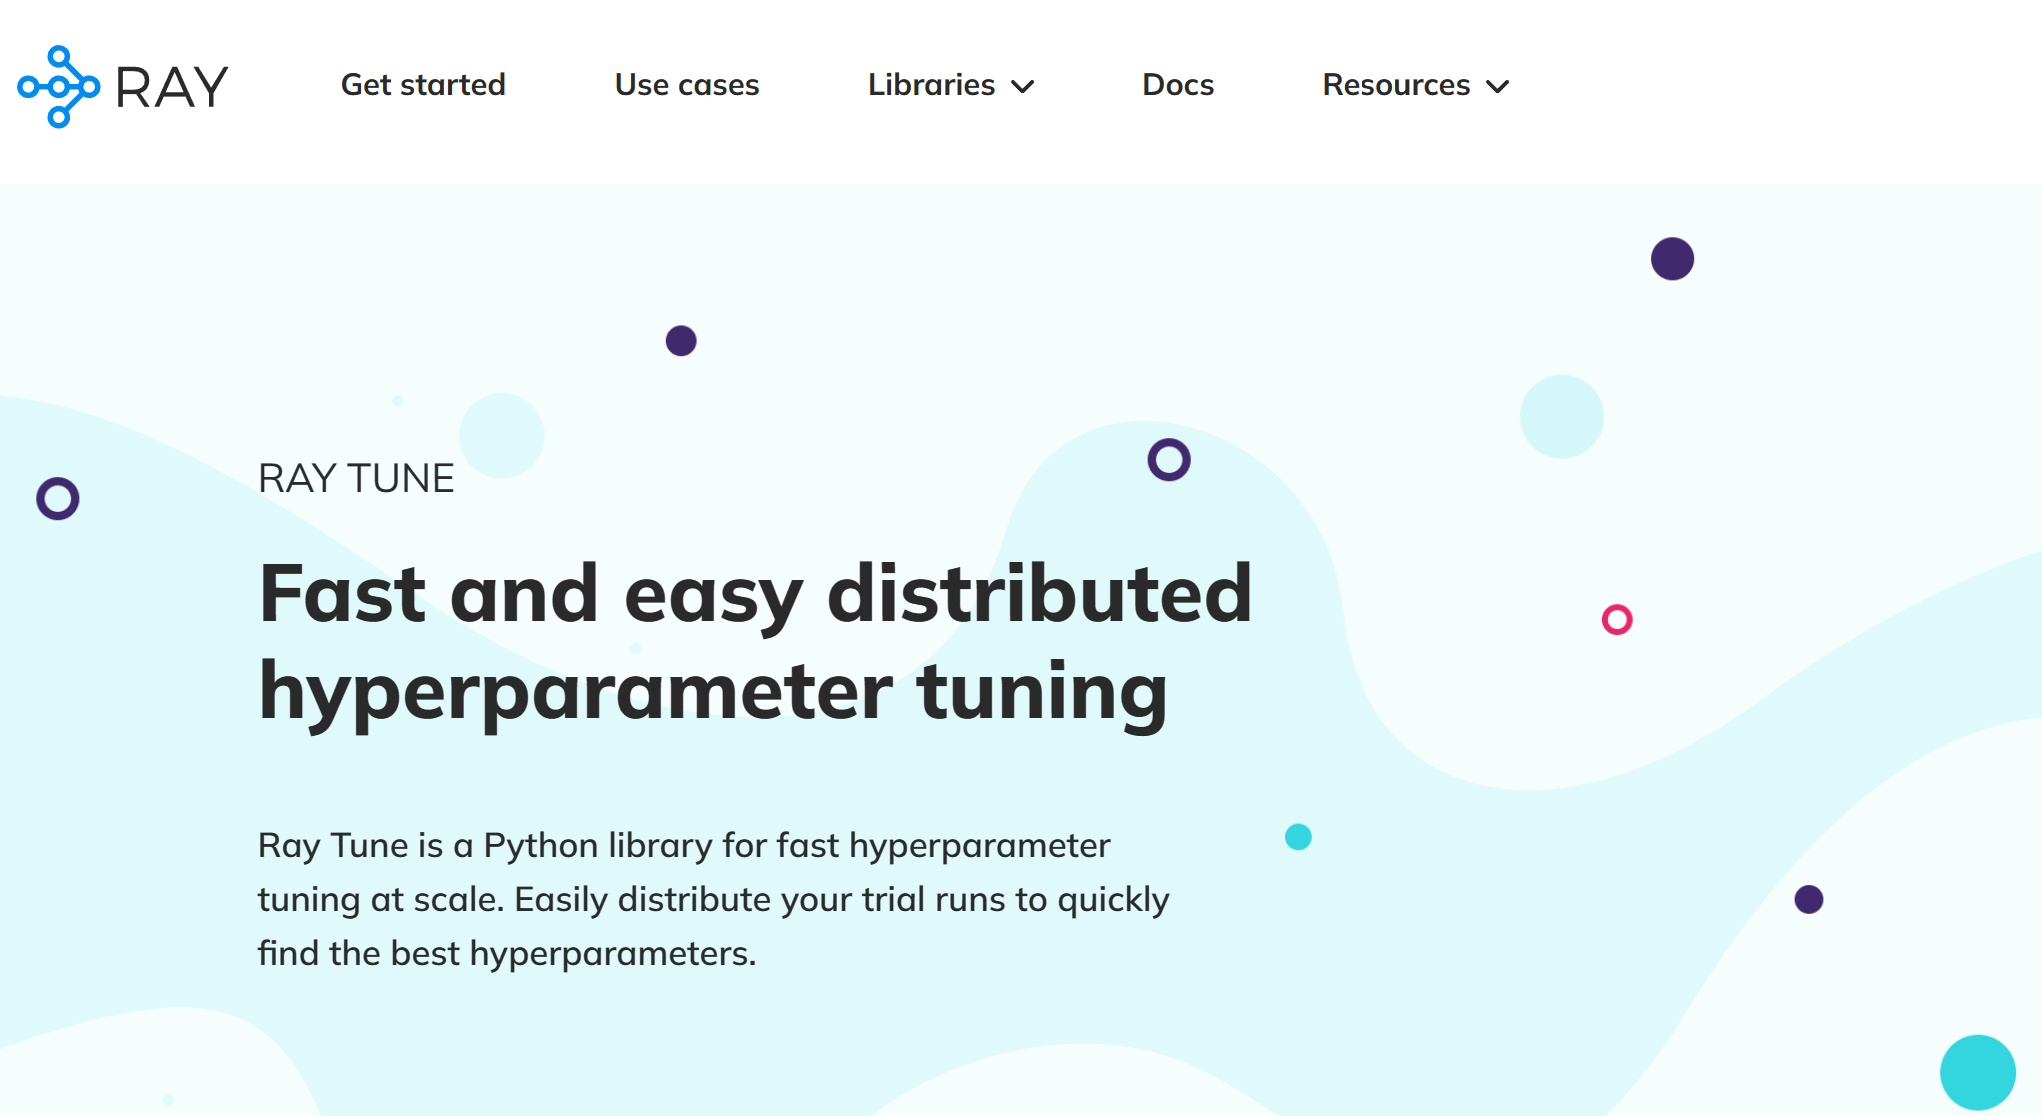
\includegraphics[width=0.95\textwidth]
			{assets/ray}
		\end{figure}
	
	\column{0.3\textwidth}
		\begin{itemize}
			\item SOTA hyperparameter tuning algorithm
			\item Easy integration in Pytorch
			\item Multi-GPU Support.
			\end{itemize}
	\end{columns}
\end{frame}

\begin{frame}
\frametitle{Ray Tune}
\framesubtitle{Easy integration in Pytorch}
		\begin{figure}
			\centering
			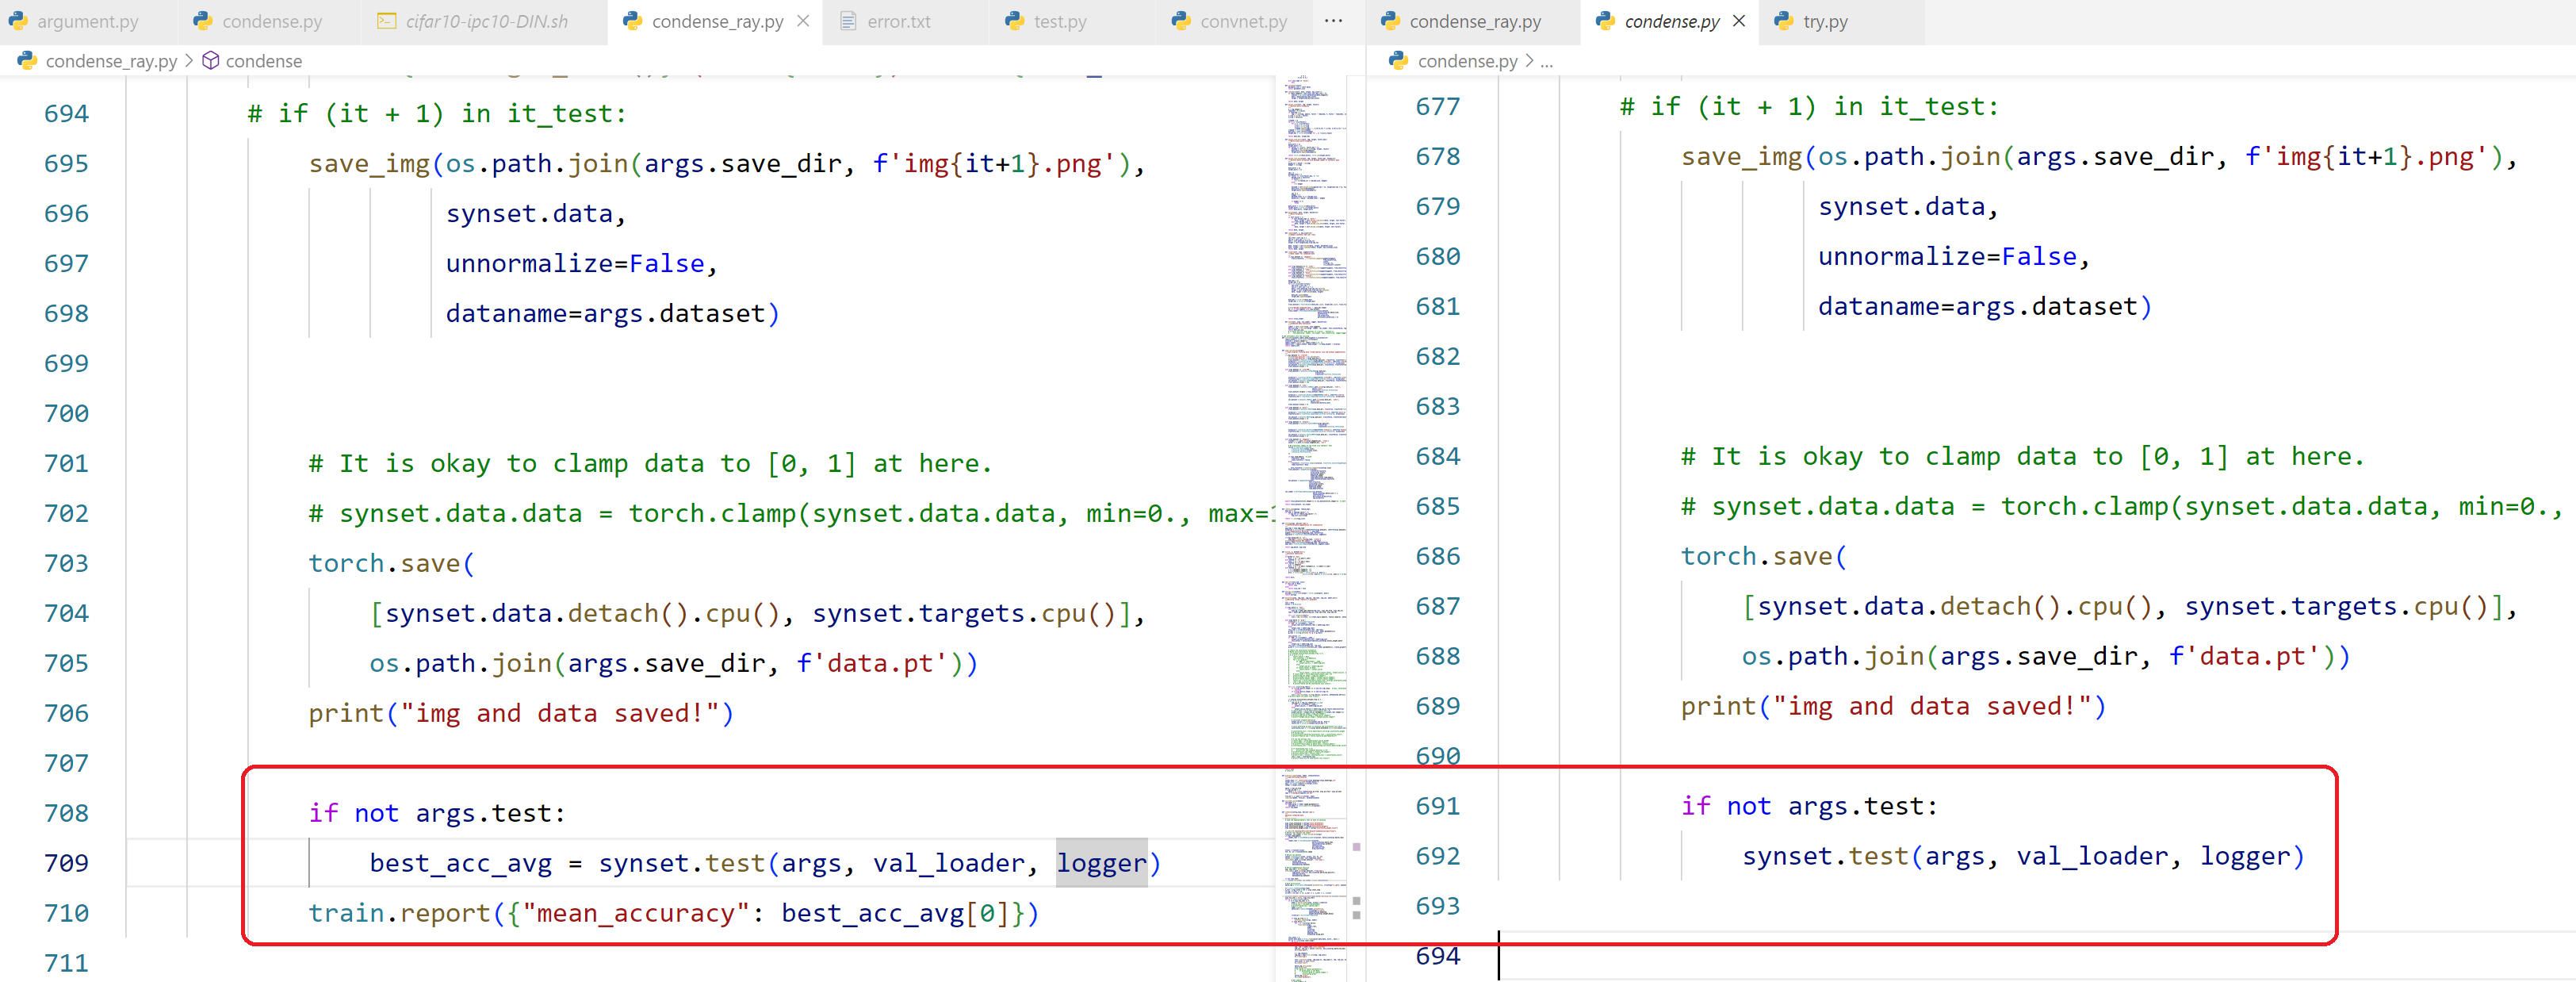
\includegraphics[width=0.9\textwidth]
			{assets/code1}
		\end{figure}
\end{frame}

\begin{frame}
\frametitle{Ray Tune}
\framesubtitle{Easy integration in Pytorch}
		\begin{figure}
			\centering
			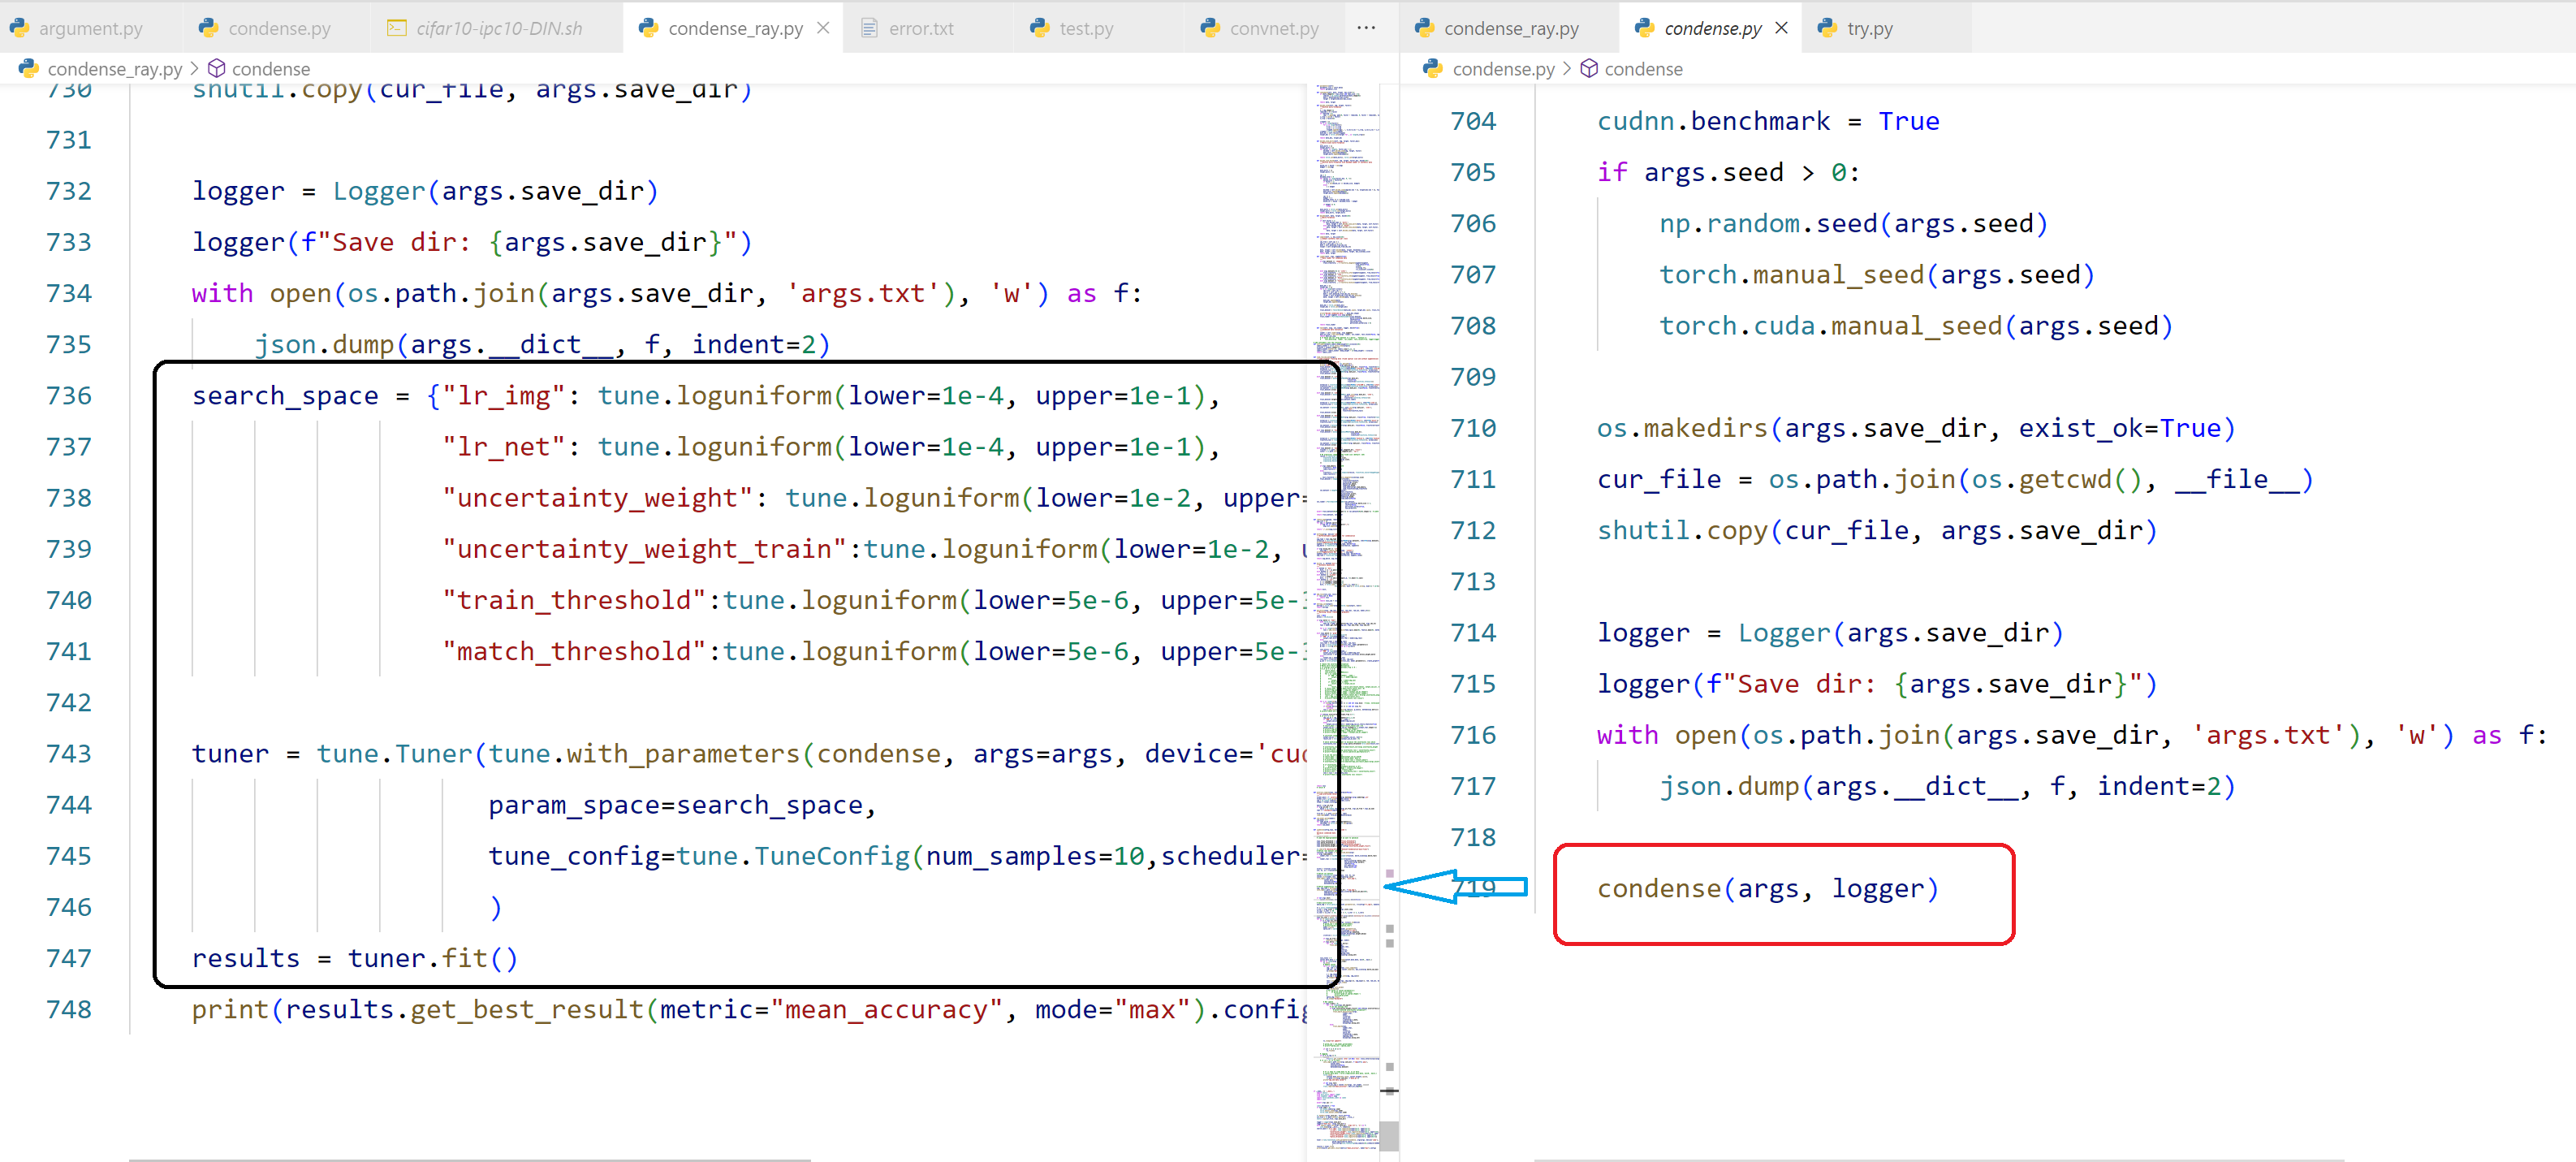
\includegraphics[width=0.9\textwidth]
			{assets/code2}
		\end{figure}
\end{frame}

\begin{frame}
\frametitle{Ray Tune}
\framesubtitle{Multi-GPU Support}
		\begin{figure}
			\centering
			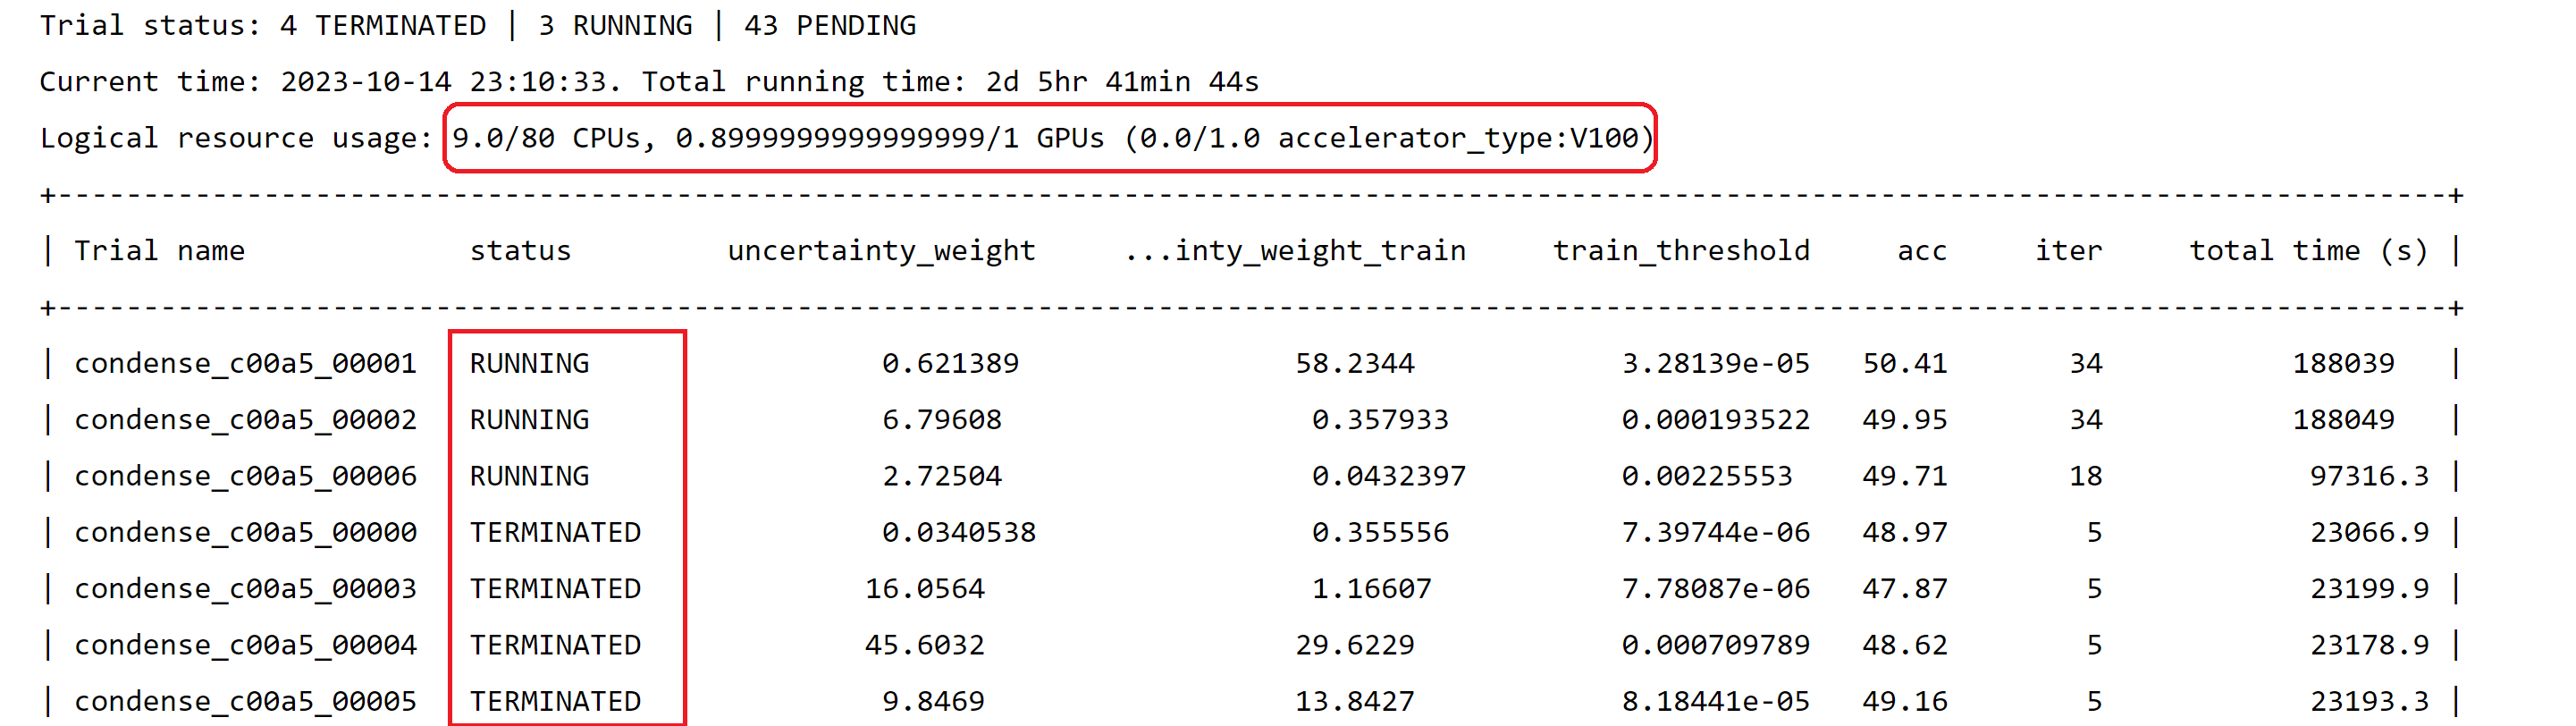
\includegraphics[width=1\textwidth]
			{assets/GPU_use}
		\end{figure}
\end{frame}




\backmatter
\end{document}
